\documentclass[11pt,fleqn, openany]{book} % Default font size and left-justified equations

%%%%%%%%%%%%%%%%%%%%%%%%%%%%%%%%%%%%%%%%%
% The Legrand Orange Book
% Structural Definitions File
% Version 2.1 (26/09/2018)
%
% Original author:
% Mathias Legrand (legrand.mathias@gmail.com) with modifications by:
% Vel (vel@latextemplates.com)
% 
% This file was downloaded from:
% http://www.LaTeXTemplates.com
%
% License:
% CC BY-NC-SA 3.0 (http://creativecommons.org/licenses/by-nc-sa/3.0/)
%
%%%%%%%%%%%%%%%%%%%%%%%%%%%%%%%%%%%%%%%%%

%----------------------------------------------------------------------------------------
%	VARIOUS REQUIRED PACKAGES AND CONFIGURATIONS
%----------------------------------------------------------------------------------------

\usepackage[table]{xcolor}

\usepackage{graphicx}
\usepackage{tabularx} % Required for including pictures
\usepackage{pgf,tikz,tkz-tab,eurosym,yhmath, stmaryrd}
\usepackage{pgfplots}
\usepackage{mathrsfs}
\usetikzlibrary{patterns}
\usetikzlibrary{trees}
\graphicspath{{../../Pictures/}}
\usepackage{multicol} 


\usepackage[english]{babel} % English language/hyphenation
\usepackage{icomma}
\usepackage{enumitem} % Customize lists
\setlist{nolistsep, nosep, nolistsep} % Reduce spacing between bullet points and numbered lists

\usepackage{booktabs} % Required for nicer horizontal rules in tables

 % Required for specifying colors by name


\definecolor{ocre}{RGB}{243,102,25} % Define the orange color used for highlighting throughout the book

\usepackage{listings}

\definecolor{codegreen}{rgb}{0,0.6,0}
\definecolor{codegray}{rgb}{0.5,0.5,0.5}
\definecolor{codepurple}{rgb}{0.58,0,0.82}
\definecolor{backcolour}{rgb}{0.95,0.95,0.92}

\lstdefinestyle{mystyle}{
    backgroundcolor=\color{backcolour},   
    commentstyle=\color{codegreen},
    keywordstyle=\color{magenta},
    numberstyle=\tiny\color{codegray},
    stringstyle=\color{codepurple},
    basicstyle=\ttfamily\footnotesize,
    breakatwhitespace=false,         
    breaklines=true,                 
    captionpos=b,                    
    keepspaces=true,                 
    numbers=left,                    
    numbersep=5pt,                  
    showspaces=false,                
    showstringspaces=false,
    showtabs=false,                  
    tabsize=2
}

\lstset{style=mystyle}

%----------------------------------------------------------------------------------------
% Paramétrage XSIM
%----------------------------------------------------------------------------------------

\usepackage[no-files]{xsim}


\DeclareExerciseEnvironmentTemplate{myex}{%
    \textbf{%
      \hypertarget{ex:\ExerciseID}{\sffamily{\ensuremath{\blacktriangleright}} Exercice \GetExerciseProperty{counter} \GetExerciseProperty{subtitle} --}
      \hyperlink{sol:\ExerciseID}{Voir le corrigé}%
    }\par
}{\par\smallskip}

\DeclareExerciseEnvironmentTemplate{mysol}{%
    \textbf{%
      \hypertarget{sol:\ExerciseID}{\sffamily{\ensuremath{\blacktriangleright}} Correction \GetExerciseProperty{counter} --}
      \hyperlink{ex:\ExerciseID}{Voir l'énoncé}%
    }\par
}{\par\medskip}

\xsimsetup{
  exercise/template = myex ,
  solution/template = mysol 
}

%Collection exercices

\DeclareExerciseTagging{topic}

\xsimsetup{collect}

%----------------------------------------------------------------------------------------
% SYMBOLES
%----------------------------------------------------------------------------------------

\newcommand\imCMsym[4][\mathord]{%
  \DeclareFontFamily{U} {#2}{}
  \DeclareFontShape{U}{#2}{m}{n}{
    <-6> #25
    <6-7> #26
    <7-8> #27
    <8-9> #28
    <9-10> #29
    <10-12> #210
    <12-> #212}{}
  \DeclareSymbolFont{CM#2} {U} {#2}{m}{n}
  \DeclareMathSymbol{#4}{#1}{CM#2}{#3}
}
\newcommand\alsoimCMsym[4][\mathord]{\DeclareMathSymbol{#4}{#1}{CM#2}{#3}}

\imCMsym{cmmi}{124}{\CMjmath}

\newcommand{\Oij}{(O\,;\,\vec{\imath}\,,\, \vec{\CMjmath} )}
\newcommand{\Oijk}{(O\,;\,\vec{\imath}\,,\, \vec{\CMjmath}\,,\,\vec{k})}

\newcommand\e{\mathrm{e}}
\newcommand\R{\mathbb{R}}
\newcommand\N{\mathbb{N}}


%----------------------------------------------------------------------------------------
%	MARGINS
%----------------------------------------------------------------------------------------

\usepackage{geometry} % Required for adjusting page dimensions and margins

\geometry{
	paper=a4paper, % Paper size, change to letterpaper for US letter size
	top=3cm, % Top margin
	bottom=3cm, % Bottom margin
	left=2cm, % Left margin
	right=2cm, % Right margin
	headheight=14pt, % Header height
	footskip=1.4cm, % Space from the bottom margin to the baseline of the footer
	headsep=10pt, % Space from the top margin to the baseline of the header
	%showframe, % Uncomment to show how the type block is set on the page
}

\setlength{\parindent}{0pt}
\parskip=5pt



%----------------------------------------------------------------------------------------
%	FONTS
%----------------------------------------------------------------------------------------

\usepackage{avant} % Use the Avantgarde font for headings
\usepackage{times} % Use the Times font for headings
\usepackage{mathptmx} % Use the Adobe Times Roman as the default text font together with math symbols from the Sym­bol, Chancery and Com­puter Modern fonts

%\usepackage{microtype} % Slightly tweak font spacing for aesthetics
%\usepackage[utf8]{inputenc} % Required for including letters with accents
\usepackage[T1]{fontenc} % Use 8-bit encoding that has 256 glyphs

%----------------------------------------------------------------------------------------
%	BIBLIOGRAPHY AND INDEX
%----------------------------------------------------------------------------------------

\usepackage[style=numeric,citestyle=numeric,sorting=nyt,sortcites=true,autopunct=true,babel=hyphen,hyperref=true,abbreviate=false,backref=true,backend=biber]{biblatex}
\addbibresource{bibliography.bib} % BibTeX bibliography file
\defbibheading{bibempty}{}

\usepackage{calc} % For simpler calculation - used for spacing the index letter headings correctly
\usepackage{makeidx} % Required to make an index
\makeindex % Tells LaTeX to create the files required for indexing

%----------------------------------------------------------------------------------------
%	MAIN TABLE OF CONTENTS
%----------------------------------------------------------------------------------------

\usepackage{titletoc} % Required for manipulating the table of contents

\contentsmargin{0cm} % Removes the default margin

% Part text styling (this is mostly taken care of in the PART HEADINGS section of this file)
\titlecontents{part}
	[0cm] % Left indentation
	{\addvspace{20pt}\bfseries} % Spacing and font options for parts
	{}
	{}
	{}

% Chapter text styling
\titlecontents{chapter}
	[1.25cm] % Left indentation
	{\addvspace{12pt}\large\sffamily\bfseries} % Spacing and font options for chapters
	{\color{ocre!60}\contentslabel[\Large\thecontentslabel]{1.25cm}\color{ocre}} % Formatting of numbered sections of this type
	{\color{ocre}} % Formatting of numberless sections of this type
	{\color{ocre!60}\normalsize\;\titlerule*[.5pc]{.}\;\thecontentspage} % Formatting of the filler to the right of the heading and the page number

% Section text styling
\titlecontents{section}
	[1.25cm] % Left indentation
	{\addvspace{3pt}\sffamily\bfseries} % Spacing and font options for sections
	{\contentslabel[\thecontentslabel]{1.25cm}} % Formatting of numbered sections of this type
	{} % Formatting of numberless sections of this type
	{\hfill\color{black}\thecontentspage} % Formatting of the filler to the right of the heading and the page number

% Subsection text styling
\titlecontents{subsection}
	[1.25cm] % Left indentation
	{\addvspace{1pt}\sffamily\small} % Spacing and font options for subsections
	{\contentslabel[\thecontentslabel]{1.25cm}} % Formatting of numbered sections of this type
	{} % Formatting of numberless sections of this type
	{\ \titlerule*[.5pc]{.}\;\thecontentspage} % Formatting of the filler to the right of the heading and the page number

% Figure text styling
\titlecontents{figure}
	[1.25cm] % Left indentation
	{\addvspace{1pt}\sffamily\small} % Spacing and font options for figures
	{\thecontentslabel\hspace*{1em}} % Formatting of numbered sections of this type
	{} % Formatting of numberless sections of this type
	{\ \titlerule*[.5pc]{.}\;\thecontentspage} % Formatting of the filler to the right of the heading and the page number

% Table text styling
\titlecontents{table}
	[1.25cm] % Left indentation
	{\addvspace{1pt}\sffamily\small} % Spacing and font options for tables
	{\thecontentslabel\hspace*{1em}} % Formatting of numbered sections of this type
	{} % Formatting of numberless sections of this type
	{\ \titlerule*[.5pc]{.}\;\thecontentspage} % Formatting of the filler to the right of the heading and the page number

%----------------------------------------------------------------------------------------
%	MINI TABLE OF CONTENTS IN PART HEADS
%----------------------------------------------------------------------------------------

% Chapter text styling
\titlecontents{lchapter}
	[0em] % Left indentation
	{\addvspace{15pt}\large\sffamily\bfseries} % Spacing and font options for chapters
	{\color{ocre}\contentslabel[\Large\thecontentslabel]{1.25cm}\color{ocre}} % Chapter number
	{}  
	{\color{ocre}\normalsize\sffamily\bfseries\;\titlerule*[.5pc]{.}\;\thecontentspage} % Page number

% Section text styling
\titlecontents{lsection}
	[0em] % Left indentation
	{\sffamily\small} % Spacing and font options for sections
	{\contentslabel[\thecontentslabel]{1.25cm}} % Section number
	{}
	{}

% Subsection text styling (note these aren't shown by default, display them by searchings this file for tocdepth and reading the commented text)
\titlecontents{lsubsection}
	[.5em] % Left indentation
	{\sffamily\footnotesize} % Spacing and font options for subsections
	{\contentslabel[\thecontentslabel]{1.25cm}}
	{}
	{}

%----------------------------------------------------------------------------------------
%	HEADERS AND FOOTERS
%----------------------------------------------------------------------------------------


\usepackage{fancyhdr} % Required for header and footer configuration

\pagestyle{fancy}
\renewcommand{\chaptermark}[1]{\markboth{\sffamily\normalsize\bfseries\ \thechapter.\ #1}{}} % Chapter text font settings
\renewcommand{\sectionmark}[1]{\markright{\sffamily\normalsize\thesection\hspace{5pt}#1}{}} % Section text font settings
\fancyhf{} \fancyhead[LE,RO]{\sffamily\normalsize\thepage} % Font setting for the page number in the header
\fancyhead[LO]{\rightmark} % Print the nearest section name on the left side of odd pages
\fancyhead[RE]{\leftmark} % Print the current chapter name on the right side of even pages

\fancyfoot[L]{Jason LAPEYRONNIE}
\fancyfoot[R]{\href{http://mathoutils.fr}{http://mathoutils.fr}} % Uncomment to include a footer

\renewcommand{\headrulewidth}{0.5pt} % Thickness of the rule under the header
\renewcommand{\footrulewidth}{0.5pt} % Thickness of the rule under the header

\fancypagestyle{plain}{% Style for when a plain pagestyle is specified
	\fancyhead{}\renewcommand{\headrulewidth}{0pt}%
}

% Removes the header from odd empty pages at the end of chapters
\makeatletter
\renewcommand{\cleardoublepage}{
\clearpage\ifodd\c@page\else
\hbox{}
\vspace*{\fill}
\thispagestyle{empty}
\newpage
\fi}

%----------------------------------------------------------------------------------------
%	THEOREM STYLES
%----------------------------------------------------------------------------------------

\usepackage{amsmath,amsfonts,amssymb,amsthm} % For math equations, theorems, symbols, etc

\newcommand{\intoo}[2]{\mathopen{]}#1\,;#2\mathclose{[}}
\newcommand{\ud}{\mathop{\mathrm{{}d}}\mathopen{}}
\newcommand{\intff}[2]{\mathopen{[}#1\,;#2\mathclose{]}}
\renewcommand{\qedsymbol}{$\blacksquare$}
\newtheorem{notation}{Notation}[section]

% Boxed/framed environments
\newtheoremstyle{ocrenumbox}% Theorem style name
{0pt}% Space above
{0pt}% Space below
{\normalfont}% Body font
{}% Indent amount
{\small\bf\sffamily\color{ocre}}% Theorem head font
{\;:\;}% Punctuation after theorem head
{0.25em}% Space after theorem head
{\small\sffamily\color{ocre}\thmname{#1}\nobreakspace\thmnumber{\@ifnotempty{#1}{}\@upn{#2}}% Theorem text (e.g. Theorem 2.1)
\thmnote{\nobreakspace\the\thm@notefont\sffamily\bfseries\color{black}---\nobreakspace#3}} % Optional theorem note

\newtheoremstyle{blacknumex}% Theorem style name
{5pt}% Space above
{10pt}% Space below
{\normalfont}% Body font
{} % Indent amount
{\small\bf\sffamily}% Theorem head font
{\;:\;}% Punctuation after theorem head
{0.25em}% Space after theorem head
{\small\sffamily{\tiny\ensuremath{\blacksquare}}\nobreakspace\thmname{#1}\nobreakspace\thmnumber{\@ifnotempty{#1}{}\@upn{#2}}% Theorem text (e.g. Theorem 2.1)
\thmnote{\nobreakspace\the\thm@notefont\sffamily\bfseries---\nobreakspace#3}}% Optional theorem note

\newtheoremstyle{blacknumexo}% Theorem style name
{15pt}% Space above
{10pt}% Space below
{\normalfont}% Body font
{} % Indent amount
{\small\bf\sffamily}% Theorem head font
{}% Punctuation after theorem head
{0.5em}% Space after theorem head
{\small\sffamily{\ensuremath{\blacktriangleright}}\nobreakspace\thmname{#1}\nobreakspace\thmnumber{\@ifnotempty{#1}{}\@upn{#2}}% Theorem text (e.g. Theorem 2.1)
\thmnote{\nobreakspace\the\thm@notefont\sffamily\bfseries---\nobreakspace#3} \\}% Optional theorem note



\newtheoremstyle{blacknumbox} % Theorem style name
{0pt}% Space above
{5pt}% Space below
{}% Body font
{}% Indent amount
{\large\bf\sffamily}% Theorem head font
{\;:\;}% Punctuation after theorem head
{0.25em}% Space after theorem head
{\small\sffamily\thmname{#1}\nobreakspace\thmnumber{\@ifnotempty{#1}{}\@upn{#2}}% Theorem text (e.g. Theorem 2.1)
\thmnote{\nobreakspace\the\thm@notefont\sffamily\bfseries---\nobreakspace#3}}% Optional theorem note

% Non-boxed/non-framed environments
\newtheoremstyle{ocrenum}% Theorem style name
{5pt}% Space above
{5pt}% Space below
{\normalfont}% Body font
{}% Indent amount
{\small\bf\sffamily\color{ocre}}% Theorem head font
{\;:\;}% Punctuation after theorem head
{0.25em}% Space after theorem head
{\small\sffamily\color{ocre}\thmname{#1}\nobreakspace\thmnumber{\@ifnotempty{#1}{}\@upn{#2}}% Theorem text (e.g. Theorem 2.1)
\thmnote{\nobreakspace\the\thm@notefont\sffamily\bfseries\color{black}---\nobreakspace#3}} % Optional theorem note
\makeatother

% Defines the theorem text style for each type of theorem to one of the three styles above
\newcounter{dummy} 
\newcounter{thm}
\newcounter{correction}
\newcounter{qst}
\theoremstyle{ocrenumbox}
\newtheorem{theoremeT}[dummy]{Théorème}
\newtheorem{exerciseT}{Propriété}
\newtheorem{principeT}{Principe}
\theoremstyle{blacknumex}
\newtheorem{exampleT}{Exemple}
\theoremstyle{blacknumexo}
\newtheorem{exo}[thm]{Exercice}
\newtheorem{corr}[correction]{Correction}
\newtheorem{quest}[qst]{Question}
\theoremstyle{blacknumbox}
\newtheorem{vocabulary}{Vocabulary}[section]
\newtheorem{definitionT}{Définition}
\newtheorem{corollaryT}[dummy]{Corollary}
\theoremstyle{ocrenum}
\newtheorem{proofT}[dummy]{Démonstration}


%----------------------------------------------------------------------------------------
%	DEFINITION OF COLORED BOXES
%----------------------------------------------------------------------------------------

\RequirePackage[framemethod=default]{mdframed} % Required for creating the theorem, definition, exercise and corollary boxes

% Theorem box
\newmdenv[skipabove=7pt,
skipbelow=7pt,
backgroundcolor=black!5,
linecolor=ocre,
innerleftmargin=5pt,
innerrightmargin=5pt,
innertopmargin=10pt,
leftmargin=0cm,
rightmargin=0cm,
innerbottommargin=5pt]{tBox}

%Proposition box	  
\newmdenv[skipabove=7pt,
skipbelow=7pt,
rightline=false,
leftline=true,
topline=false,
bottomline=false,
backgroundcolor=ocre!10,
linecolor=ocre,
innerleftmargin=5pt,
innerrightmargin=5pt,
innertopmargin=10pt,
innerbottommargin=3pt,
leftmargin=0cm,
rightmargin=0cm,
linewidth=4pt]{eBox}	

% Definition box
\newmdenv[skipabove=7pt,
backgroundcolor=ocre!4,
skipbelow=7pt,
rightline=false,
leftline=true,
topline=false,
bottomline=false,
linecolor=ocre,
innerleftmargin=5pt,
innerrightmargin=5pt,
innertopmargin=10pt,
leftmargin=0cm,
rightmargin=0cm,
linewidth=4pt,
innerbottommargin=5pt]{dBox}	

% Corollary box
\newmdenv[skipabove=7pt,
skipbelow=7pt,
rightline=false,
leftline=true,
topline=false,
bottomline=false,
linecolor=gray,
backgroundcolor=black!5,
innerleftmargin=5pt,
innerrightmargin=5pt,
innertopmargin=5pt,
leftmargin=0cm,
rightmargin=0cm,
linewidth=4pt,
innerbottommargin=5pt]{cBox}

\newmdenv[skipabove=7pt,
skipbelow=7pt,
backgroundcolor=black!5,
innerleftmargin=5pt,
topline=false,
bottomline=false,
rightline=false,
leftline=false,
innerrightmargin=5pt,
innertopmargin=5pt,
leftmargin=0cm,
rightmargin=0cm,
innerbottommargin=5pt]{xBox}

% Creates an environment for each type of theorem and assigns it a theorem text style from the "Theorem Styles" section above and a colored box from above
\newenvironment{theorem}{\begin{tBox}\begin{theoremeT}}{\end{theoremeT}\end{tBox}}

\newenvironment{exo2}{\noindent \begin{exo}\item\relax \noindent \begin{eBox}\item\relax}{\end{eBox}\end{exo}}


\newenvironment{proposition}{\begin{eBox}\begin{exerciseT}}{\hfill{\color{ocre}}\end{exerciseT}\end{eBox}}		

\newenvironment{principe}{\begin{eBox}\begin{principeT}}{\hfill{\color{ocre}}\end{principeT}\end{eBox}}	
		  
\newenvironment{definition}{\begin{dBox}\begin{definitionT}}{\end{definitionT}\end{dBox}}	

\newenvironment{example}{\begin{xBox}\begin{exampleT}}{\hfill{\tiny\ensuremath{\blacksquare}}\end{exampleT}\end{xBox}}

\newenvironment{demonstration}{\begin{proofT}}{\hfill{\tiny\ensuremath{\square}}\end{proofT}}		
\newenvironment{corollary}{\begin{cBox}\begin{corollaryT}}{\end{corollaryT}\end{cBox}}	

%----------------------------------------------------------------------------------------
%	REMARK ENVIRONMENT
%----------------------------------------------------------------------------------------

\newenvironment{remark}{\par\vspace{5pt}\small % Vertical white space above the remark and smaller font size
\begin{list}{}{
\leftmargin=25pt % Indentation on the left
\rightmargin=15pt}\item\ignorespaces % Indentation on the right
\makebox[-2.5pt]{
\begin{tikzpicture}[overlay]
\node[draw=ocre!60,line width=1pt,circle,fill=ocre!25,font=\sffamily\bfseries,inner sep=2pt,outer sep=0pt] at (-15pt,0pt){\textcolor{ocre}{R}};\end{tikzpicture}} % Orange R in a circle
\advance\baselineskip -1pt}{\end{list}\vskip5pt} % Tighter line spacing and white space after remark

%----------------------------------------------------------------------------------------
%	SECTION NUMBERING IN THE MARGIN
%----------------------------------------------------------------------------------------

\makeatletter
\renewcommand{\@seccntformat}[1]{\llap{\textcolor{ocre}{\csname the#1\endcsname}\hspace{1em}}}                    
\renewcommand{\section}{\@startsection{section}{1}{\z@}
{-4ex \@plus -1ex \@minus -.4ex}
{1ex \@plus.2ex }
{\normalfont\LARGE\sffamily\bfseries}}
\renewcommand{\subsection}{\@startsection {subsection}{2}{\z@}
{-3ex \@plus -0.1ex \@minus -.4ex}
{0.5ex \@plus.2ex }
{\normalfont\sffamily\bfseries}}
\renewcommand{\subsubsection}{\@startsection {subsubsection}{3}{\z@}
{-2ex \@plus -0.1ex \@minus -.2ex}
{.2ex \@plus.2ex }
{\normalfont\small\sffamily\bfseries}}                        
\renewcommand\paragraph{\@startsection{paragraph}{4}{\z@}
{-2ex \@plus-.2ex \@minus .2ex}
{.1ex}
{\normalfont\small\sffamily\bfseries}}

%----------------------------------------------------------------------------------------
%	PART HEADINGS
%----------------------------------------------------------------------------------------

% Numbered part in the table of contents
\newcommand{\@mypartnumtocformat}[2]{%
	\setlength\fboxsep{0pt}%
	\noindent\colorbox{ocre!20}{\strut\parbox[c][.7cm]{\ecart}{\color{ocre!70}\Large\sffamily\bfseries\centering#1}}\hskip\esp\colorbox{ocre!40}{\strut\parbox[c][.7cm]{\linewidth-\ecart-\esp}{\Large\sffamily\centering#2}}%
}

% Unnumbered part in the table of contents
\newcommand{\@myparttocformat}[1]{%
	\setlength\fboxsep{0pt}%
	\noindent\colorbox{ocre!40}{\strut\parbox[c][.7cm]{\linewidth}{\Large\sffamily\centering#1}}%
}

\newlength\esp
\setlength\esp{4pt}
\newlength\ecart
\setlength\ecart{1.2cm-\esp}
\newcommand{\thepartimage}{}%
\newcommand{\partimage}[1]{\renewcommand{\thepartimage}{#1}}%
\def\@part[#1]#2{%
\ifnum \c@secnumdepth >-2\relax%
\refstepcounter{part}%
\addcontentsline{toc}{part}{\texorpdfstring{\protect\@mypartnumtocformat{\thepart}{#1}}{\partname~\thepart\ ---\ #1}}
\else%
\addcontentsline{toc}{part}{\texorpdfstring{\protect\@myparttocformat{#1}}{#1}}%
\fi%
\startcontents%
\markboth{}{}%
{\thispagestyle{empty}%
\begin{tikzpicture}[remember picture,overlay]%
\node at (current page.north west){\begin{tikzpicture}[remember picture,overlay]%	
\fill[ocre!20](0cm,0cm) rectangle (\paperwidth,-\paperheight);
\node[anchor=north] at (4cm,-3.25cm){\color{ocre!40}\fontsize{220}{100}\sffamily\bfseries\thepart}; 
\node[anchor=south east] at (\paperwidth-1cm,-\paperheight+1cm){\parbox[t][][t]{8.5cm}{
\printcontents{l}{0}{\setcounter{tocdepth}{1}}% The depth to which the Part mini table of contents displays headings; 0 for chapters only, 1 for chapters and sections and 2 for chapters, sections and subsections
}};
\node[anchor=north east] at (\paperwidth-1.5cm,-3.25cm){\parbox[t][][t]{15cm}{\strut\raggedleft\color{white}\fontsize{30}{30}\sffamily\bfseries#2}};
\end{tikzpicture}};
\end{tikzpicture}}%
\@endpart}
\def\@spart#1{%
\startcontents%
\phantomsection
{\thispagestyle{empty}%
\begin{tikzpicture}[remember picture,overlay]%
\node at (current page.north west){\begin{tikzpicture}[remember picture,overlay]%	
\fill[ocre!20](0cm,0cm) rectangle (\paperwidth,-\paperheight);
\node[anchor=north east] at (\paperwidth-1.5cm,-3.25cm){\parbox[t][][t]{15cm}{\strut\raggedleft\color{white}\fontsize{30}{30}\sffamily\bfseries#1}};
\end{tikzpicture}};
\end{tikzpicture}}
\addcontentsline{toc}{part}{\texorpdfstring{%
\setlength\fboxsep{0pt}%
\noindent\protect\colorbox{ocre!40}{\strut\protect\parbox[c][.7cm]{\linewidth}{\Large\sffamily\protect\centering #1\quad\mbox{}}}}{#1}}%
\@endpart}
\def\@endpart{\vfil\newpage
\if@twoside
\if@openright
\null
\thispagestyle{empty}%
\newpage
\fi
\fi
\if@tempswa
\twocolumn
\fi}

%----------------------------------------------------------------------------------------
%	CHAPTER HEADINGS
%----------------------------------------------------------------------------------------

% A switch to conditionally include a picture, implemented by Christian Hupfer
\newif\ifusechapterimage
\usechapterimagetrue
\newcommand{\thechapterimage}{}%
\newcommand{\chapterimage}[1]{\ifusechapterimage\renewcommand{\thechapterimage}{#1}\fi}%
\newcommand{\autodot}{.}
\def\@makechapterhead#1{%
{\parindent \z@ \raggedright \normalfont
\ifnum \c@secnumdepth >\m@ne
\if@mainmatter
\begin{tikzpicture}[remember picture,overlay]
\node at (current page.north west)
{\begin{tikzpicture}[remember picture,overlay]
\node[anchor=north west,inner sep=0pt] at (0,0) {\ifusechapterimage\includegraphics[width=\paperwidth]{\thechapterimage}\fi};
\draw[anchor=west] (\Gm@lmargin,-3cm) node [line width=2pt,rounded corners=15pt,draw=ocre,fill=white,fill opacity=0.5,inner sep=15pt]{\strut\makebox[22cm]{}};
\draw[anchor=west] (\Gm@lmargin+.3cm,-3cm) node {\huge\sffamily\bfseries\color{black}\thechapter\autodot~#1\strut};
\end{tikzpicture}};
\end{tikzpicture}
\else
\begin{tikzpicture}[remember picture,overlay]
\node at (current page.north west)
{\begin{tikzpicture}[remember picture,overlay]
\node[anchor=north west,inner sep=0pt] at (0,0) {\ifusechapterimage\includegraphics[width=\paperwidth]{\thechapterimage}\fi};
\draw[anchor=west] (\Gm@lmargin,-3cm) node [line width=2pt,rounded corners=15pt,draw=ocre,fill=white,fill opacity=0.5,inner sep=15pt]{\strut\makebox[22cm]{}};
\draw[anchor=west] (\Gm@lmargin+.3cm,-3cm) node {\huge\sffamily\bfseries\color{black}#1\strut};
\end{tikzpicture}};
\end{tikzpicture}
\fi\fi\par\vspace*{50\p@}}}

%-------------------------------------------

\def\@makeschapterhead#1{%
\begin{tikzpicture}[remember picture,overlay]
\node at (current page.north west)
{\begin{tikzpicture}[remember picture,overlay]
\node[anchor=north west,inner sep=0pt] at (0,0) {\ifusechapterimage\includegraphics[width=\paperwidth]{\thechapterimage}\fi};
\draw[anchor=west] (\Gm@lmargin,-3cm) node [line width=2pt,rounded corners=15pt,draw=ocre,fill=white,fill opacity=0.5,inner sep=15pt]{\strut\makebox[22cm]{}};
\draw[anchor=west] (\Gm@lmargin+.3cm,-3cm) node {\huge\sffamily\bfseries\color{black}#1\strut};
\end{tikzpicture}};
\end{tikzpicture}
\par\vspace*{50\p@}}
\makeatother

%----------------------------------------------------------------------------------------
%	LINKS
%----------------------------------------------------------------------------------------

\usepackage{hyperref}
\hypersetup{hidelinks,backref=true,pagebackref=true,hyperindex=true,colorlinks=false,breaklinks=true,urlcolor=ocre,bookmarks=true,bookmarksopen=false}

\usepackage{bookmark}
\bookmarksetup{
open,
numbered,
addtohook={%
\ifnum\bookmarkget{level}=0 % chapter
\bookmarksetup{bold}%
\fi
\ifnum\bookmarkget{level}=-1 % part
\bookmarksetup{color=ocre,bold}%
\fi
}
}

\renewcommand*\thesection{\arabic{section}}

\newcommand*{\coord}[3]{% 
  \ensuremath{\overrightarrow{#1}\, 
    \begin{pmatrix} 
      #2\\ 
      #3 
    \end{pmatrix}}}
    
  \newcommand*{\coordb}[2]{% 
  \ensuremath{ 
    \begin{pmatrix} 
      #1\\ 
      #2 
    \end{pmatrix}}}

\newcommand*{\coorde}[4]{% 
  \renewcommand{\arraystretch}{1}\ensuremath{\overrightarrow{#1}\, 
    \begin{pmatrix} 
      #2\\ 
      #3 \\
      #4
    \end{pmatrix}}}    
  \newcommand*{\coordbe}[3]{% 
 \renewcommand{\arraystretch}{1} \ensuremath{ 
    \begin{pmatrix} 
      #1\\ 
      #2 \\
      #3
    \end{pmatrix}}}  
    
\newcommand{\Card}{\mathrm{Card}}



\begin{document}

\chapterimage{../../Pictures/background}


\chapter{Cours : Orthogonalité dans l'espace}


\section{Produit scalaire de deux vecteurs}


\subsection{Définition du produit scalaire}


\begin{definition}Soient $\vec u$ et $\vec v$ deux vecteurs de l'espace. On considère des points $A$, $B$ et $C$ tels que $\vec u = \overrightarrow{AB}$ et $\vec v= \overrightarrow{AC}$. L'angle non orienté entre les vecteurs $\vec u$ et $\vec v$, noté $(\vec u;\vec v)$ est  l'angle $\widehat{BAC}$, vu dans le plan $(ABC)$.\end{definition}

\begin{definition}Le produit scalaire de $\vec u$ et $\vec v$ est le \textbf{réel} notée $\vec u \cdot \vec v$ et qui vaut
\begin{itemize}
\item 0 si $\vec u$ ou $\vec v$ vaut $\overrightarrow{0}$ ;
\item $\lvert\lvert\vec u\rvert\rvert \times \lvert\lvert\vec v\rvert\rvert \times \cos (\vec u ; \vec v)$ sinon.
\end{itemize}\end{definition}

\textbf{Rappel de certaines valeurs remarquables}

\begin{center}
\renewcommand{\arraystretch}{2.5}
\noindent \begin{tabularx}{0.9\linewidth}{|X|XXXXXX|}
\hline
Degré & 0 & 30 & 45 & 60 & 90 & 180 \\
\hline
Radians & 0 & $\dfrac{\pi}{6}$ & $\dfrac{\pi}{4}$ & $\dfrac{\pi}{3}$ & $\dfrac{\pi}{2}$ & $\pi$ \\
\hline
Cosinus & 1 & $\dfrac{\sqrt{3}}{2}$ & $\dfrac{\sqrt{2}}{2}$ & $\dfrac{1}{2}$ & 0 & -1\\
\hline
Sinus & 0 & $\dfrac{1}{2}$ & $\dfrac{\sqrt{2}}{2}$ & $\dfrac{\sqrt{3}}{2}$ & 1 & 0\\
\hline
\end{tabularx}
\end{center}




\begin{example} Dans un cube $ABCDEFGH$ de côté 1, calculer le produit scalaire $\overrightarrow{AD} \cdot \overrightarrow{BG}$.

\begin{minipage}{0.3\linewidth}
\begin{center}
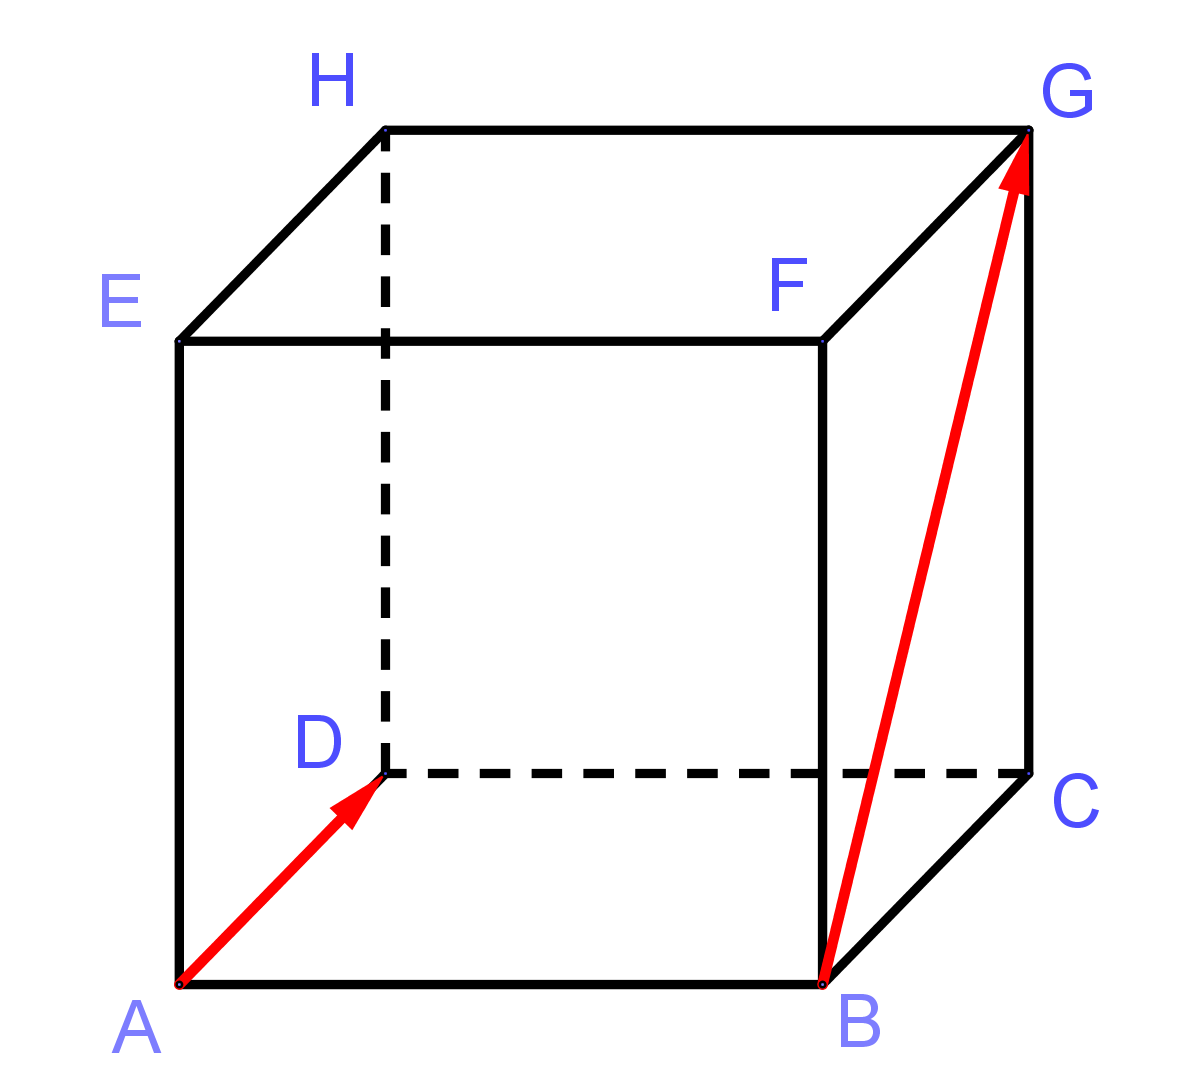
\includegraphics[scale=0.7]{cube4}
\end{center}
\end{minipage}\hfill\begin{minipage}{0.65\linewidth}
D'une part, $\overrightarrow{BG}=\overrightarrow{AH}$. Ainsi, $\overrightarrow{AD} \cdot \overrightarrow{BG} = \overrightarrow{AD} \cdot \overrightarrow{AH}$.

L'angle $\widehat{HAD}$ mesure 45$^\circ$ ou $\dfrac{\pi}{4}$ radians.

$AD=1$. Le théorème de Pythagore permet de montrer que $AH=\sqrt{2}$.

Ainsi, $\overrightarrow{AD} \cdot \overrightarrow{AH}= AD \times AH \times \cos \left( \dfrac{\pi}{4}\right) = 1 \times \sqrt{2} \times \dfrac{\sqrt{2}}{2}=1$.
\end{minipage}

\end{example}

\begin{definition}On dit que deux vecteurs $\vec u$ et $\vec v$ sont orthogonaux si $\vec u \cdot \vec v=0$.
\end{definition}

Le vecteur $\vec 0$ est en particulier orthogonal à tous les autres vecteurs.

\newpage
\subsection{Propriétés du produit scalaire}

\begin{proposition}Soit $\vec u$, $\vec v$ et $\vec w$ trois vecteurs de l'espace, $k$ et $k'$ deux réels.
\begin{itemize}
\item $\vec u \cdot \vec u = \lvert\lvert \vec u\rvert\rvert^2$. En particulier, $\lvert\lvert\vec u\rvert\rvert=\sqrt{\vec u \cdot \vec u}$.
\item $\vec u \cdot \vec v = \vec v \cdot \vec u$, le produit scalaire est \textbf{symétrique}.
\item $\vec u \cdot ( k \vec v + k' \vec w)= k (\vec u \cdot \vec v) + k' (\vec u \cdot \vec w)$ et $( k \vec v + k' \vec w)\cdot \vec u= k (\vec v \cdot \vec u) + k' (\vec w \cdot \vec u)$. \\Le produit scalaire est \textbf{bilinéaire}.
\end{itemize}\end{proposition}

\begin{example} Soit $\vec u$, $\vec v$ et $\vec w$ trois vecteurs tels que $\vec u \cdot \vec v = 3$, $\vec v \cdot \vec w=5$, $\vec u \cdot \vec w = -1$ et $\lvert\lvert\vec u\rvert\rvert=4$. On a
\[ (\vec u + 2\vec v) \cdot (-3\vec u + 4 \vec w)=-3 (\vec u \cdot \vec u) + 4 (\vec u \cdot \vec w) - 6 (\vec v \cdot \vec u) + 8 (\vec v \cdot \vec w).\]
On remplace alors les valeurs par celle de l'énoncé en rappelant que $\vec u \cdot \vec u = \lvert\lvert\vec u\rvert\rvert^2$.
\[ (\vec u + 2\vec v) \cdot (-3\vec u + 4 \vec w)=-3 \times 4^2 + 4 \times (-1) - 6 \times 3 + 8\times 5=-30\]\vspace{-0.5cm}\end{example}

\subsection{Formules de polarisation}

\begin{proposition}Soit $\vec u$ et $\vec v$ deux vecteurs de l'espace.
\begin{itemize}
\item $(\vec{u}+\vec{v})^2=\lvert\lvert\vec{u}\rvert\rvert^2+2\vec{u}\cdot\vec{v}+\lvert\lvert\vec{v}\rvert\rvert^2$ ;
\item $(\vec{u}-\vec{v})^2=\lvert\lvert\vec{u}\rvert\rvert^2-2\vec{u}\cdot\vec{v}+\lvert\lvert\vec{v}\rvert\rvert^2$ ;
\item $(\vec{u}+\vec{v})\cdot (\vec{u}-\vec{v})=\lvert\lvert\vec{u}\rvert\rvert^2-\lvert\lvert\vec{v}\rvert\rvert^2$.
\end{itemize}\end{proposition}

\begin{demonstration} On utilise la bilinéarité du produit scalaire. On a\[(\vec{u}+\vec{v})^2 =  (\vec{u}+\vec{v}) \cdot (\vec{u}+\vec{v})= \vec{u}\cdot\vec{u}+\vec{u}\cdot \vec{v}+\vec{v}\cdot\vec{u}+\vec{v}\cdot \vec{v}=\lvert\lvert\vec{u}\rvert\rvert^2+2\vec{u}\cdot\vec{v}+\lvert\lvert\vec{v}\rvert\rvert^2.\]
\[(\vec{u}-\vec{v})^2 =  (\vec{u}-\vec{v}) \cdot (\vec{u}-\vec{v})= \vec{u}\cdot\vec{u}-\vec{u}\cdot \vec{v}-\vec{v}\cdot\vec{u}+\vec{v}\cdot \vec{v}=\lvert\lvert\vec{u}\rvert\rvert^2-2\vec{u}\cdot\vec{v}+\lvert\lvert\vec{v}\rvert\rvert^2.\]
\[(\vec{u}+\vec{v})\cdot (\vec{u}-\vec{v})= \vec{u}\cdot\vec{u}-\vec{u}\cdot \vec{v}+\vec{v}\cdot\vec{u}-\vec{v}\cdot \vec{v}=\lvert\lvert\vec{u}\rvert\rvert^2-\lvert\lvert\vec{v}\rvert\rvert^2.\]
\end{demonstration}

\begin{proposition}Soit $\vec{u}$ et $\vec{v}$ deux vecteurs de l'espace.
\begin{itemize}
\item $\vec{u} \cdot \vec{v}= \dfrac{1}{2}(\lvert\lvert\vec{u}+\vec{v}\rvert\rvert^2-\lvert\lvert\vec{u}\rvert\rvert^2-\lvert\lvert\vec{v}\rvert\rvert^2)$ ;
\item $\vec{u} \cdot \vec{v}= -\dfrac{1}{2}(\lvert\lvert\vec{u}-\vec{v}\rvert\rvert^2-\lvert\lvert\vec{u}\rvert\rvert^2-\lvert\lvert\vec{v}\rvert\rvert^2)$ ;
\item $\vec{u} \cdot \vec{v} = \dfrac{1}{4}( \lvert\lvert\vec{u}+\vec{v}\rvert\rvert^2-\lvert\lvert\vec{u}-\vec{v}\rvert\rvert^2 )$.
\end{itemize}\end{proposition}

\begin{demonstration} Soit $\vec{u}$ et $\vec{v}$ deux vecteurs du plan. D'après la propriété précédente, on a 
\[\lvert\lvert\vec{u}+\vec{v}\rvert\rvert^2=\lvert\lvert\vec{u}\rvert\rvert^2+2\vec{u}\cdot\vec{v}+\lvert\lvert\vec{v}\rvert\rvert^2\quad\text{et}\quad \lvert\lvert\vec{u}-\vec{v}\rvert\rvert^2=\lvert\lvert\vec{u}\rvert\rvert^2-2\vec{u}\cdot\vec{v}+\lvert\lvert\vec{v}\rvert\rvert^2.\]
En isolant $\vec{u}\cdot \vec{v}$ dans ces deux expressions, on retrouve les deux premiers points. De plus, en soustrayant ces deux égalités, on trouve que
\[\lvert\lvert\vec{u}+\vec{v}\rvert\rvert^2-\lvert\lvert\vec{u}-\vec{v}\rvert\rvert^2=4\vec{u}\cdot\vec{v}.\]
Il suffit de diviser par 4 pour retrouver la dernière égalité recherchée.\end{demonstration}

\begin{example}Soit $A$, $B$ et $C$ trois points de l'espace tels que $AB=5$, $BC=7$ et $AC=8$. On a
\[\overrightarrow{AB}\cdot \overrightarrow{AC}=-\dfrac{1}{2}( \lvert\lvert\overrightarrow{AB}-\overrightarrow{AC}\rvert\rvert^2-AB^2-AC^2).\]
Or, $\overrightarrow{AB}-\overrightarrow{AC}=\overrightarrow{AB}+\overrightarrow{CA}=\overrightarrow{CB}$, d'où
\[\overrightarrow{AB}\cdot \overrightarrow{AC}=-\dfrac{1}{2}( CB^2-AB^2-AC^2)=-\dfrac{1}{2}(7^2-5^2-8^2)=-20.\]\vspace{-0.5cm}\end{example}


\section{Base orthonormée}

\begin{definition}Soit $\Oijk$ un repère de l'espace.
\begin{itemize}
\item On dit que la base $(\vec{\imath}, \vec{\CMjmath}, \vec k)$ est orthonormée si
\begin{itemize}
\item $\vec{\imath} \cdot \vec{\CMjmath} = \vec{\imath} \cdot \vec k = \vec{\CMjmath} \cdot \vec k = 0$ ;
\item $\lvert\lvert\vec{\imath}\rvert\rvert=\lvert\lvert\vec{\CMjmath}\rvert\rvert=\lvert\lvert\vec k\rvert\rvert = 1$.
\end{itemize}
\item On dit alors que le repère $\Oijk$ est un repère orthonormé.
\end{itemize}\end{definition}

Une famille orthonormée de trois vecteurs forme forcément une base de l'espace.

\begin{example} Si on considère un cube $ABCDEFGH$ de côté 1, le repère $(A;\overrightarrow{AB},\overrightarrow{AD}, \overrightarrow{AE})$ est un repère orthonormé de l'espace.\end{example}

\begin{proposition}On se place dans un repère orthonormé $\Oijk$. 

On considère deux vecteurs \renewcommand{\arraystretch}{1}\coorde{u}{x}{y}{z} et \renewcommand{\arraystretch}{1}\coorde{v}{x'}{y'}{z'}. Alors, $\vec u \cdot \vec v =xx'+yy'+zz'$.\end{proposition}

\begin{demonstration} Il suffit de revenir à la définition de coordonnées. On a
\[ \vec u \cdot \vec v = (x\vec{\imath} + y \vec{\CMjmath} + z \vec k) \cdot (x' \vec{\imath} + y' \vec{\CMjmath} + z' \vec k).\]
On développe alors
\[ \vec u \cdot \vec v = xx' \vec{\imath} \cdot \vec{\imath} +  xy' \vec{\imath} \cdot \vec{\CMjmath} +  xz' \vec{\imath} \cdot \vec k +  yx' \vec{\CMjmath} \cdot \vec{\imath} +  yy' \vec{\CMjmath} \cdot \vec{\CMjmath} +  yz' \vec{\CMjmath} \cdot \vec k +  zx' \vec k \cdot \vec{\imath} +  zy' \vec k \cdot \vec{\CMjmath} +  zz' \vec k \cdot \vec k .\]
Or, la base $(\vec{\imath}, \vec{\CMjmath}, \vec k)$ est orthonormé, les seuls produits scalaires non nuls sont $\vec{\imath} \cdot \vec{\imath}$, $\vec{\CMjmath} \cdot \vec{\CMjmath}$, et $\vec k \cdot \vec k$ qui valent 1. Ainsi, 
\[ \vec u \cdot \vec v =xx'+yy'+zz'.\]\vspace{-0.5cm}\end{demonstration}

\begin{example} Dans un repère orthonormé $\Oijk$, on considère les vecteurs \renewcommand{\arraystretch}{1}\coorde{u}{3}{-1}{2} et \renewcommand{\arraystretch}{1}\coorde{v}{5}{3}{-6}.
\[ \vec u \cdot \vec v = 3 \times 5 + (-1) \times 3 + 2 \times -6 = 15 -3 -12=0.\]
Les vecteurs $\vec u$ et $\vec v$ sont orthogonaux.\end{example}

\begin{proposition} On se place dans un repère orthonormé $\Oijk$. Soit \renewcommand{\arraystretch}{1}\coorde{u}{x}{y}{z} un vecteur de l'espace. 

Alors $ \lvert\lvert\vec u\rvert\rvert = \sqrt{ \vec u \cdot \vec u} =  \sqrt{x^2+y^2+z^2}$.

En particulier, si $A(x_A,y_A,z_A)$ et $B(x_B, y_B, z_B)$ sont deux points de l'espace, alors
\[ AB = \sqrt{(x_B-x_A)^2+(y_B-y_A)^2+(z_B-z_A)^2} .\]\end{proposition}

\begin{example} On se place dans un repère orthonormé $\Oijk$. Soit $A(1;2;5)$ et $B(3;3;3)$. On a alors
\[ AB = \sqrt{(3-1)^2+(3-2)^2+(3-5)^2}=\sqrt{2^2+1^2+2^2}=\sqrt{9}=3.\]\end{example}



\section{Orthogonalité}

\subsection{Droites orthogonales}

\begin{definition}Soit $(d)$ et $(d')$ deux droites de l'espace. On dit que $(d)$ et $(d')$ sont orthogonales si les parallèles à ces deux droites passant par un même point sont perpendiculaires.\end{definition}

\begin{example} On considère un cube $ABCDEFGH$.

\begin{center}
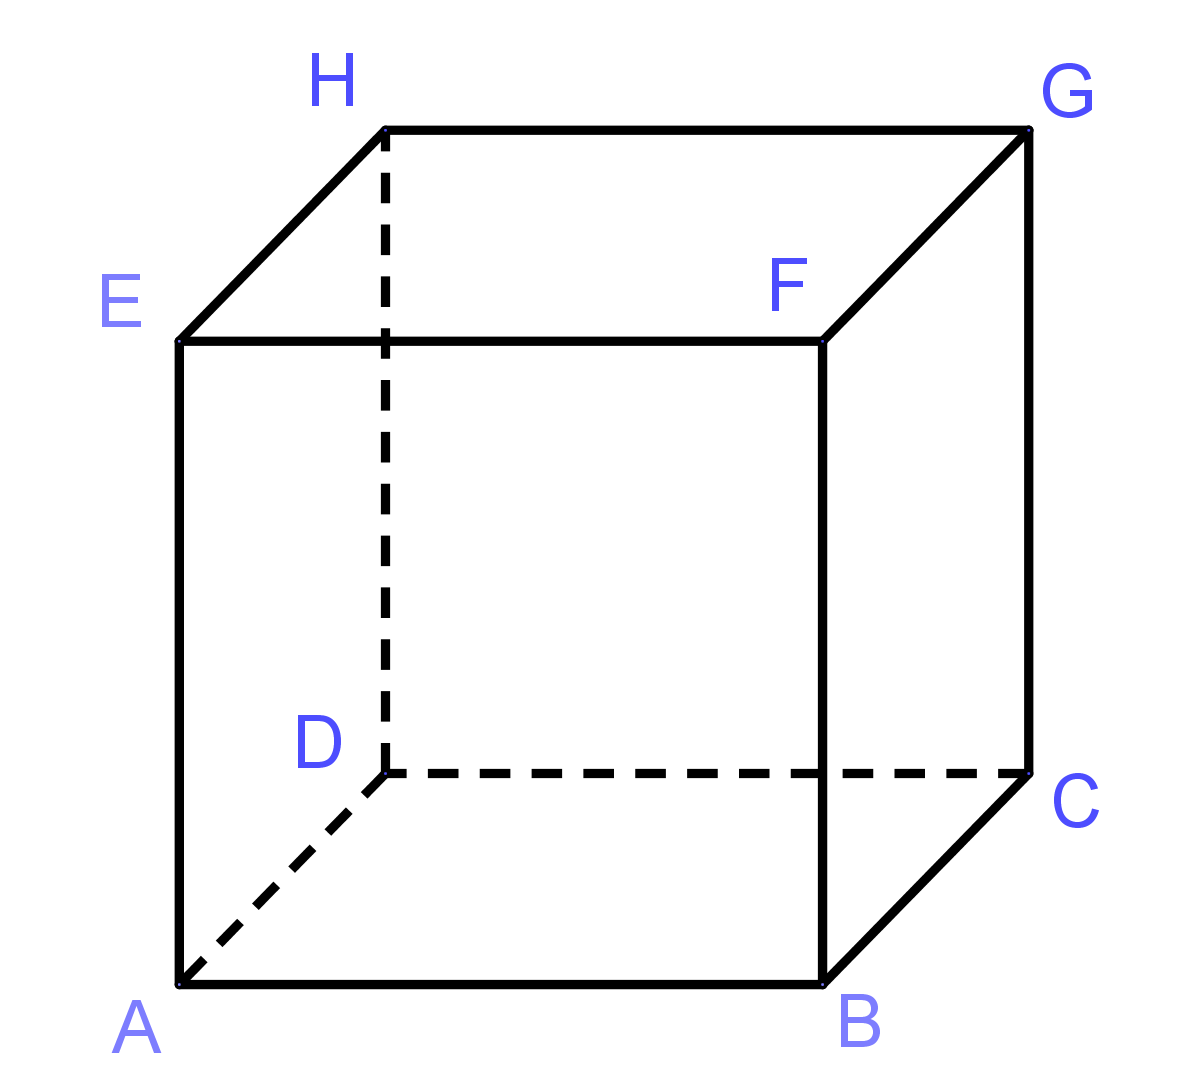
\includegraphics[scale=1]{cube}
\end{center}

Les droites $(AB)$ et $(CG)$ sont orthogonales. En effet, la parallèle à $(CG)$ passant par $B$ est la droite $(BF)$ qui est perpendiculaire à la droite $(AB)$.\end{example}
\newpage
\begin{proposition}Deux droites $(d)$ et $(d')$, dirigées respectivement par les vecteurs $\vec u$ et $\vec v$, sont orthogonales si et seulement si $\vec u \cdot \vec v = 0$.\end{proposition}

\begin{example}On se place dans un repère orthonormé $(O,\vec{\imath}, \vec{\CMjmath}, \vec k)$. On considère les droites $(d_1)$ et $(d_2)$ définies par les représentations paramétriques suivantes.

\[ (d_1)\, ; \, \left\{ \renewcommand{\arraystretch}{1}\begin{array}{l}x=1-2t\\y=3+t\\z=2-t\end{array}\right. \quad \text{et} \quad (d_2)\, ; \, \left\{ \renewcommand{\arraystretch}{1}\begin{array}{l}x=5-3t\\y=3-2t\\z=2+4t\end{array}\right.\]

La droite $(d_1)$ est dirigée par le vecteur $\renewcommand{\arraystretch}{1}\coorde{u}{-2}{1}{-1}$ et la droite $(d_2)$  par le vecteur $\renewcommand{\arraystretch}{1}\coorde{v}{-3}{-2}{4}$.

Le repère étant orthonormé, on peut calculer le produit scalaire de ces deux vecteurs comme suit :\[ \vec u \cdot \vec v = -2 \times (-3) + 1 \times (-2) + (-1) \times 4 = 6-2-4=0.\]
Les vecteurs $\vec u$ et $\vec v$ sont orthogonaux. Les droites $(d_1)$ et $(d_2)$ sont donc orthogonales.\end{example}

\subsection{Droite orthogonale à un plan}

\begin{definition}Soit $(d)$ une droite et $\mathcal{P}$ un plan de l'espace. On dit que $(d)$ est orthogonale au plan $\mathcal{P}$ si elle est orthogonale à toute droite contenue dans le plan $\mathcal{P}$.\end{definition}

\begin{proposition}[Théorème de la porte]Soit $(d)$ une droite de vecteur directeur $\vec u$ et $\mathcal{P}$ un plan de l'espace dirigé par les vecteurs $\vec v_1$ et $\vec v_2$. La droite $(d)$ est orthogonale au plan $\mathcal{P}$ si et seulement si $\vec u \cdot \vec v_1 = \vec u \cdot \vec v_2 = 0$.\end{proposition}

Il suffit donc de montrer qu'une droite est orthogonale à deux droites sécantes d'un plan pour montrer qu'elle est en fait orthogonale à toute droites de ce plan.


\begin{example} On se place dans un repère orthonormé $\Oijk$. 

On considère les vecteurs \renewcommand{\arraystretch}{1}\coorde{v_1}{1}{2}{3} et \renewcommand{\arraystretch}{1}\coorde{v_2}{1}{0}{1} ainsi que deux points $A(2;5;2)$ et $B(5;8;-1)$.

On note $\mathcal{P}$ le plan passant par le point $O$ et dirigé par les vecteurs $\vec v_1$ et $\vec v_2$ (ces vecteurs n'étant pas colinéaires, on définit bien ainsi un plan). La droite $(AB)$ est orthogonale au plan $\mathcal{P}$. En effet,
\begin{itemize}
\item Le vecteur $\overrightarrow{AB}$ a pour coordonnées \renewcommand{\arraystretch}{1}\coorde{AB}{3}{3}{-3}
\item Puisque l'on est dans un repère orthonormé, on peut calculer les produits scalaires à l'aide des coordonnées. On a alors
\begin{itemize}
\item $\overrightarrow{AB} \cdot  v_1 = 3 \times 1 + 3 \times 2 + (-3) \times 3 = 0$ ;
\item $\overrightarrow{AB} \cdot v_2 = 3 \times 1 + 3 \times 0 + (-3) \times 1 = 0$.
\end{itemize}
\item Ainsi, $\overrightarrow{AB}$ est orthogonal aux vecteurs $\vec v_1$ et $\vec v_2$. La droite $(AB)$ est donc orthogonale au plan $\mathcal{P}$.
\end{itemize}\end{example}



\subsection{Vecteur normal à un plan}

\begin{definition}Soit $\mathcal{P}$ un plan et $\vec n$ un vecteur non nul.
On dit que $\vec n$ est un vecteur normal au plan $\mathcal{P}$ s'il est orthogonal à tout vecteur directeur du plan $\mathcal{P}$.\end{definition}

De la même manière que ce que l'on faisait avec les droites orthogonales à un plan, pour montrer qu'un vecteur est normal à un plan, il suffit de montrer qu'il est orthogonal à deux vecteurs non colinéaires de ce plan.

\begin{example}On se place dans un repère orthonormé $\Oijk$. On considère le plan $\mathcal{P}$ passant par $O$ et dirigé par les vecteurs \renewcommand{\arraystretch}{1}\coorde{v_1}{3}{2}{6} et \renewcommand{\arraystretch}{1}\coorde{v_2}{1}{-3}{2}. Le vecteur \renewcommand{\arraystretch}{1}\coorde{u}{2}{0}{-1} est  normal au plan $\mathcal{P}$. En effet,
\begin{itemize}
\item Les vecteurs $\vec{v_1}$ et $\vec{v}_2$ ne sont pas colinéaires. Ils définissent donc bien un plan.
\item Puisque l'on est dans un repère orthonormé, il est possible de calculer le produit scalaire à l'aide des coordonnées,
\item $ \vec u \cdot \vec v_1 = 2 \times 3 + 0 \times 2 + (-1) \times 6 = 0$ ;
\item $\vec u \cdot \vec v_2 = 2 \times 1 + 0 \times (-3) + (-1) \times 2 = 0$.
\end{itemize}
Ainsi, $\vec u$ est orthogonal à $\vec v_1$ et $\vec v_2$. $\vec u$ est donc un vecteur normal au plan $\mathcal{P}$.\end{example}

\begin{proposition}Deux plans sont parallèles si et seulement si un vecteur normal au premier est normal au second.\end{proposition}

\begin{example}On se place dans un repère orthonormé $\Oijk$. 

On considère le plan $\mathcal{P}_2$ passant par $A(2;5;9)$, dirigé par \renewcommand{\arraystretch}{1}\coorde{w_1}{5}{4}{10} et \renewcommand{\arraystretch}{1}\coorde{w_2}{-2}{7}{-4}. 

Le vecteur \renewcommand{\arraystretch}{1}\coorde{u}{2}{0}{-1}, qui était normal au plan $\mathcal{P}$ de l'exemple précédent, est aussi normal au plan $\mathcal{P}_2$.\\ En effet, les vecteurs $\vec{w_1}$ et $\vec{w}_2$ ne sont pas colinéaires et définissent donc bien un plan.
De plus, puisque l'on est dans un repère orthonormé, il est possible de calculer le produit scalaire à l'aide des coordonnées,
\begin{itemize}\item $ \vec u \cdot \vec w_1 = 2 \times 5 + 0 \times 4 + (-1) \times 10 = 0$ ;
\item $\vec u \cdot \vec w_2 = 2 \times (-2) + 0 \times 7 + (-1) \times (-4) = 0$.
\end{itemize}
Ainsi, $\vec u$ est orthogonal à $\vec w_1$ et $\vec w_2$. $\vec u$ est donc un vecteur normal au plan $\mathcal{P}_2$. Les plans $\mathcal{P}$ et $\mathcal{P}_2$ admettent un même vecteur normal, ils sont donc parallèles.\end{example}


\begin{definition}Deux plans sont perpendiculaires si le premier plan contient une droite orthogonale au second plan.\end{definition}

Le concept de plans perpendiculaires peut être trompeur. Par exemple, deux plans perpendiculaires peuvent contenir des droites parallèles. En revanche, il est possible de caractériser la perpendicularité de deux plans en utilisant leurs vecteurs normaux.

\begin{proposition} Deux plans sont perpendiculaires si un vecteur normal à l'un est orthogonal à un vecteur normal du second.
\end{proposition}


\newpage

\section{Equation cartésienne d'un plan}

Dans toute cette partie et dans la suivante, l'espace est muni d'un repère orthonormé $\Oijk$.

\subsection{Equation cartésienne}

\begin{proposition}Soit $\vec n$ un vecteur de l'espace et $A$ un point de l'espace. L'ensemble des points $M$ tel que $\overrightarrow{AM}\cdot \vec{n}=0$ est le plan passant par $A$ admettant le vecteur $\vec n$ comme vecteur normal.

Réciproquement, soit $\mathcal{P}$ un plan de l'espace, $A$ un point de $\mathcal{P}$ et $\vec n$ un vecteur normal à $\mathcal{P}$. $\mathcal{P}$ est l'ensemble des points $M$ tels que $\overrightarrow{AM} \cdot \vec n=0$.\end{proposition}

Il est donc possible de décrire un plan à l'aide d'un point et d'un vecteur normal.

\begin{proposition}Soit $A (x_A,y_A,z_A)$ un point de l'espace et $\renewcommand{\arraystretch}{1}\coorde{n}{a}{b}{c}$ un vecteur non nul.

On note $\mathcal{P}$ le plan passant par le point $A$ et admettant le vecteur $\vec n$ comme vecteur normal.

Un point $M(x,y,z)$ appartient au plan $\mathcal{P}$ si et seulement si\[ a(x-x_A)+b(y-y_A)+c(z-z_A)=0.\]

Cette équation est appelée équation cartésienne du plan $\mathcal{P}$.


Réciproquement, si $a$, $b$, $c$ et $d$ sont quatre réels fixés, avec $(a,b,c)\neq (0,0,0)$, l'ensemble des points $M(x;y;z)$ vérifiant $ax+by+cz+d=0$ est un plan auquel le vecteur \renewcommand{\arraystretch}{1}\coorde{n}{a}{b}{c} est  normal.\end{proposition}

\begin{demonstration} Soit $M(x;y;z)$ un point de l'espace. Le point $M$ appartient au plan $\mathcal{P}$ passant par $A (x_A,y_A,z_A)$ et de vecteur normal \renewcommand{\arraystretch}{1}\coorde{n}{a}{b}{c} si et seulement si $\overrightarrow{AM}\cdot \vec n =0$. Puisque le repère que l'on considère est orthonormé,
\[\overrightarrow{AM}\cdot \vec n =  \renewcommand{\arraystretch}{1}\coordbe{x-x_A}{y-y_A}{z-z_A} \cdot \renewcommand{\arraystretch}{1}\coordbe{a}{b}{c}= a(x-x_A)+b(y-y_A)+c(z-z_A).\]
Ainsi, le point $M$ appartient au plan $\mathcal{P}$ si et seulement si $ a(x-x_A)+b(y-y_A)+c(z-z_A)=0$.

Réciproquement, $a$, $b$, $c$ et $d$ quatre réels fixés, avec $(a,b,c)\neq (0,0,0)$. On supposera par exemple que $a\neq 0$. On note alors $\vec n$ le vecteur de coordonnées $\renewcommand{\arraystretch}{1}\coordbe{a}{b}{c}$.

D'une part, l'ensemble $\mathcal{E}$ des points de l'espace vérifiant $ax+by+cz+d=0$ n'est pas vide. En effet, le point $A\left( -\frac{d}{a} ; 0 ; 0\right)$ appartient à cet ensemble. 

Soit $M(x;y;z)$ un point de l'espace et $A \in \mathcal{E}$. On a alors $ax_A+by_A+cz_A=-d$. Ainsi, 
\[ M\in \mathcal{E} \Leftrightarrow ax+by+cz+d=0 \Leftrightarrow ax+by+cz-ax_a-by_A-cz_A=0 \Leftrightarrow a(x-x_A)+b(y-y_A)+c(z-z_A)=0 \]

C'est-à-dire $M \in \mathcal{E}$ si et seulement si $\overrightarrow{AM} \cdot \vec n = 0$. L'ensemble $\mathcal{E}$ est donc un plan admettant $\vec n$ comme vecteur normal.\end{demonstration}


\begin{example}On considère le plan $\mathcal{P}$ d'équation cartésienne $3x+2y-3z+1=0$. Ce plan admet le vecteur $\vec n\renewcommand{\arraystretch}{1}\renewcommand{\arraystretch}{1}\begin{pmatrix}3\\2\\-3\end{pmatrix}$ comme vecteur normal.

Considérons le point $A(1;1;2)$. On a $3 \times 1 + 2 \times 1 - 3 \times 2 + 1 =0$. Les coordonnées du point $A$ vérifient l'équation du plan $\mathcal{P}$. Le point $A$ appartient donc au plan $\mathcal{P}$.

En revanche, le point $B(1;5;0)$ n'appartient pas à ce plan : on a $3 \times 1 + 2 \times 5 - 3 \times 0 +1 = 14 \neq 0$.\end{example}


\begin{example} Le plan $\mathcal{P}$ passant par $A(1;5;7)$ et admettant le vecteur \renewcommand{\arraystretch}{1}\coorde{n}{4}{-2}{3} a pour équation cartésienne $4(x-1)-2(y-5)+3(z-7)=0$ c'est-à-dire $4x-2y+3z-15=0$.\end{example}
Il est aussi possible de raisonner comme suit : tout plan admettant le vecteur \renewcommand{\arraystretch}{1}\coorde{n}{4}{-2}{3} comme vecteur normal admet une équation cartésienne de la forme $4x-2y+3z+d=0$ pour un certain réel $d$. Pour que ce plan passe par le point $A$, il faut que les coordonnées de $A$ vérifient cette équation.

Autrement dit, $4 \times 1 -2 \times 5 + 3 \times 7 + d =0$, soit $15+d=0$ et donc $d=-15$.





\subsection{Application : intersection d'une droite et d'un plan}



\begin{example}On considère le plan $\mathcal{P}$ d'équation $2x+5y-3z+1=0$ et la droite $(d)$ de représentation paramétrique  $\left\{ \begin{array}{l}x=2-t \\ y=5+t \\ z = -2-2t \\\end{array}\right., t \in \mathbb{R}$. Soit $M(x;y;z)$ un point de l'espace.

On a $M(x;y;z)\in P \cap (d)$ si et seulement s'il existe un réel  $t$ tel que $\left\{ \begin{array}{l}x=2-t \\ y=5+t \\ z = -2-2t \\2x+5y-3z+1=0 \end{array}\right.$

Résolvons ce système. En remplaçant les valeurs de $x$, $y$ et $z$ dans la dernière équation, on obtient
\[ \left\{ \begin{array}{l}x=2-t \\ y=5+t \\ z = -2-2t \\2(2-t)+5(5+t)-3(-2-2t)+1=0 \end{array}\right.\quad  \text{soit}\quad \left\{ \begin{array}{l}x=2-t \\ y=5+t \\ z = -2-2t \\36+9t=0 \end{array}\right.\]
Finalement, l'unique solution du système est
\[ \left\{ \begin{array}{l}t=-4 \\x=2-(-4)=6 \\ y=5+(-4)=1 \\ z = -2-2 \times (-4)=6 \end{array}\right.\]
L'intersection de $\mathcal{P}$ et $(d)$ est donc le point $M(6;1;6)$.\end{example}



\section{Projeté orthogonal}

\subsection{Projeté orthogonal sur une droite}

\begin{definition}Soit $A$ un point de l'espace et $(d)$ une droite de l'espace, dirigée par un vecteur $\vec u$.
On appelle projeté orthogonal de $A$ sur $(d)$ le point $H$ de la droite $(d)$ tel que $\overrightarrow{AH} \cdot \vec{u}=0$. En particulier,
\begin{itemize}
\item Si $A$ appartient à la droite $(d)$, ce point est son propre projeté,
\item sinon, la droite $(AH)$ est perpendiculaire à la droite $(d)$.
\end{itemize}\end{definition}

\begin{center}
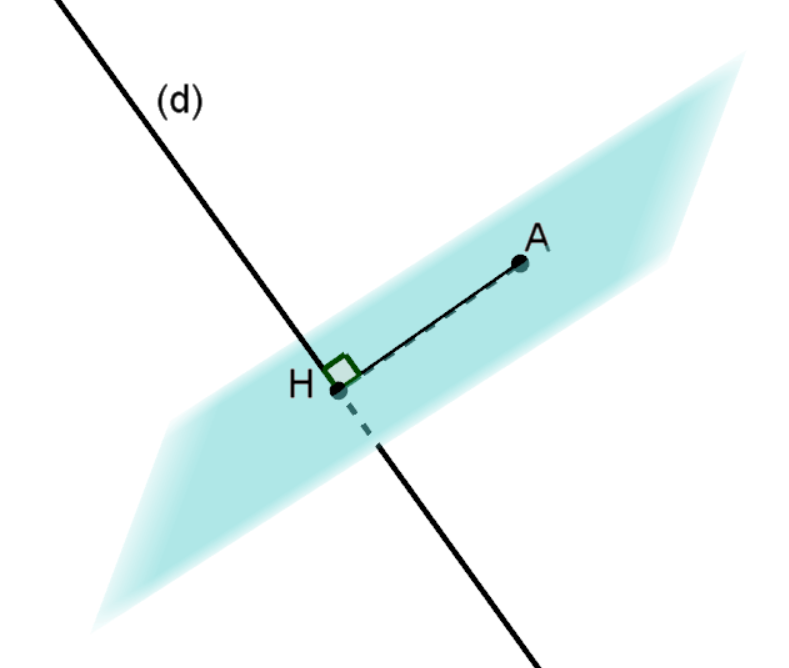
\includegraphics[scale=0.3]{projort}
\end{center}

$H$ est en fait l'intersection de la droite $(d)$ et du plan $\mathcal{P}$ qui passe par le point $A$ et auquel la droite $(d)$ est normale. Si l'on connaît un point et un vecteur directeur de la droite $(d)$, il est alors possible de déterminer sa représentation paramétrique, déterminer l'équation cartésienne du plan $\mathcal{P}$, puis d'en déterminer le point d'intersection avec la méthode vue précédemment : nous déterminons ainsi le projeté orthogonal de $A$ sur $(d)$.

\begin{example}Soit $(d)$ la droite de représentation paramétrique  $\left\{ \begin{array}{l}x=1-t \\ y=3+t \\ z = 1-2t \\\end{array}\right., t \in \mathbb{R}$ et $A$ le point de coordonnées $(3;3;3)$. On vérifie facilement que le point $A$ n'appartient pas à la droite $(d)$.

Un vecteur directeur de la droite $(d)$ est le vecteur $\vec n\renewcommand{\arraystretch}{1}\begin{pmatrix}-1\\1\\-2\end{pmatrix}$. Notons alors $\mathcal{P}$ le plan passant par $A$ est donc $\vec u$ est un vecteur normal : la droite $(d)$ sera ainsi orthogonale à ce plan $\mathcal{P}$. 

Une équation cartésienne du plan $\mathcal{P}$ est donc \[-(x-3)+(y-3)-2(z-3)=0\quad\text{soit}\quad -x+y-2z+6=0.\] Le projeté orthogonal de $A$ sur $(d)$ est le point d'intersection de $(d)$ et de $\mathcal{P}$.

Notons $(x;y;z)$ les coordonnées de ce point et $t$ son paramètre dans l'équation de $(d)$. On a alors $x=1-t$, $y=3+t$, $z=1-2t$ et $-x+y-2z+6=0$. En remplaçant les valeurs de $x$, $y$ et $z$ dans cette dernière équation, on aboutit alors à \[-(1-t)+(3+t)-2(1-2t)+6=0\quad \text{soit}\quad 6t+6=0 \quad \text{et donc}\quad t=-1.\]

Ainsi, $x=1-(-1)=2$, $y=3+(-1)=2$ et $z=1-2\times(-1)=3$. Le projeté orthogonal du point $A$ sur la droite $(d)$ est donc le point $H(2;2;3)$.\end{example}

\subsection{Projeté orthogonal sur un plan}
\begin{definition}Soit $A$ un point de l'espace, $\mathcal{P}$ un plan de l'espace et $\vec n$ un vecteur normal de $\mathcal{P}$. Le projeté orthogonal de $A$ sur $\mathcal{P}$ est le point d'intersection $H$ du plan $\mathcal{P}$ et de la droite passant par $A$ et dirigée par le vecteur $\vec n$. En particulier
\begin{itemize}
\item Si $A$ appartient au plan $\mathcal{P}$, ce point est son propre projeté
\item sinon, le vecteur $\overrightarrow{AH}$ est normal au plan $\mathcal{P}$
\end{itemize}\end{definition}

\begin{center}
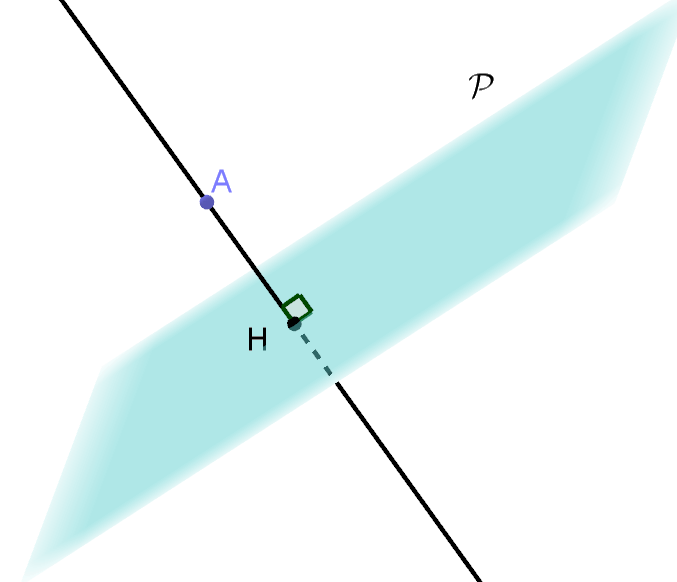
\includegraphics[scale=0.3]{projort2}
\end{center}


\begin{example} On se place dans un repère orthonormé $\Oijk$. On considère le point $A$ de coordonnées $(1;3;6)$, le point $B$ de coordonnées $(1;1;1)$ et le plan $\mathcal{P}$ passant par $B$ et dirigé par \renewcommand{\arraystretch}{1}\coorde{v_1}{1}{0}{0} et \renewcommand{\arraystretch}{1}\coorde{v_2}{1}{10}{-4}. Ces deux vecteurs n'étant pas colinéaires, on définit bien ainsi un plan.

\begin{itemize}
\item Les coordonnées du vecteur $\overrightarrow{AB}$ sont $\renewcommand{\arraystretch}{1}\coorde{AB}{0}{-2}{-5}$.
\item Puisque l'on est dans un repère orthonormé, il est possible de calculer le produit scalaire à l'aide des coordonnées,
\begin{itemize}
\item $\overrightarrow{AB}\cdot \vec v_1 = 0 \times 1 + (-2) \times 0 + (-5) \times 0 = 0$ ;
\item $\overrightarrow{AB}\cdot \vec v_1 = 0 \times 2 + (-2) \times 10 + (-5) \times (-4) = 0$ ;
\end{itemize}
\item Ainsi, $B$ appartient au plan $\mathcal{P}$ et le vecteur $\overrightarrow{AB}$ est normal au plan $\mathcal{P}$. $B$ est donc le projeté orthogonal de $A$ sur $\mathcal{P}$.
\end{itemize}\end{example}

Là encore, une méthode similaire à la précédente peut être utilisée pour déterminer par le calcul les coordonnées du projeté orthogonal d'un point sur un plan. Si l'on connaît l'équation cartésienne d'un plan $\mathcal{P}$ ainsi que les coordonnées d'un point $A$ n'appartenant pas à ce plan, il est possible de déterminer les coordonnées du projeté orthogonal de $A$ sur $\mathcal{P}$. 

Pour cela, on identifie un vecteur $\vec n$ normal à $\mathcal{P}$ et on détermine une représentation paramétrique de la droite passant par $A$ et admettant $\vec n$ comme vecteur directeur : cette droite est orthogonale au plan $\mathcal{P}$. Il nous reste alors à déterminer les coordonnées du point d'intersection de cette droite et de ce plan pour obtenir le projeté orthogonal de $A$ sur $\mathcal{P}$.

\newpage
\subsection{Distance à une droite ou un plan}

\begin{definition}Soit $A$ un point de l'espace et $(d)$ une droite (ou $\mathcal{P}$ un plan). 

On appelle distance de $A$ à $(d)$ (ou à $\mathcal{P}$) la plus petite distance $AM$ pour $M$ un point de la droite $(d)$ (ou du plan $\mathcal{P}$).\end{definition}

\begin{example}Soit $A(2,1,3)$ et $(d)$ la droite de représentation paramétrique $\left\{ \begin{array}{l}x=1-t \\ y=5+t \\ z = -2-2t \\\end{array}\right., t \in \mathbb{R}$. \\Soit $M$ un point de paramètre $t$ de cette droite. On a alors
\[AM^2=(2-(1-t))^2+(1-(5+t))^2+(3-(-2-2t))^2=(1+t)^2+(-4-t)^2+(5+2t)^2.\]
Développons alors cette expression. On a
\[AM^2=1+2t+t^2+16+8t+t^2+25+20t+4t^2=6t^2+30t+42.\]
Ainsi, $AM=\sqrt{6t^2+30t+42}$. Or, pour tout réel $t$, $6t^2+30t+42>0$. On rappelle que si $u$ est une fonction définie, dérivable et strictement positive sur $\mathbb{R}$, alors la fonction $\sqrt{u}$ est dérivable sur $\mathbb{R}$ et $(\sqrt{u})'=\dfrac{u'}{2\sqrt{u}}$. Ainsi, la fonction $f:x\mapsto \sqrt{6t^2+30t+42}$ est donc définie et dérivable sur $\mathbb{R}$ et, pour tout réel $t$, 
\[f'(t)= \dfrac{12t+30}{2\sqrt{6t^2+30t+42}}=\dfrac{6t+15}{\sqrt{6t^2+30t+42}}.\]
Cette dérivée est du signe de $6t+15$. On sait par ailleurs que $6t+15\geqslant 0$ si et seulement si $t \geqslant - \dfrac{5}{2}$. On peut alors construire le tableau de signes de $f'$ et en déduire le tableau de variations de $f$.

\begin{center}
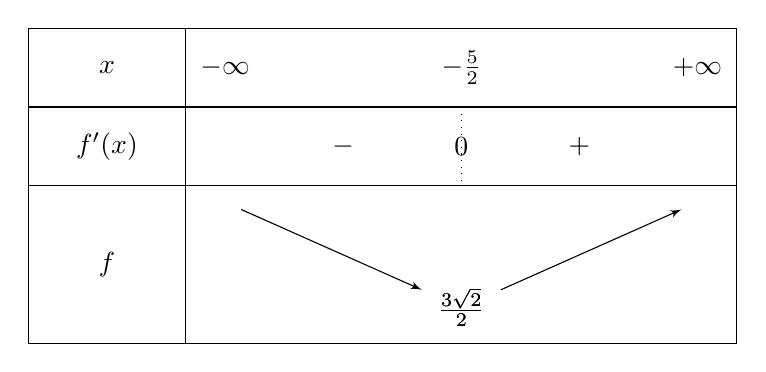
\begin{tikzpicture}[scale=1]
\tikzset{node style/.style = {inner sep = 2pt, outer sep = 2pt}}
   \tkzTabInit{$x$ / 1 , $f'(x)$/1, $f$ / 2}{$-\infty$, $-\frac{5}{2}$,$+\infty$}
      \tkzTabLine{,-,z, +, }
   \tkzTabVar{+/$ $,-/$\frac{3\sqrt{2}}{2}$,+/$ $}
\end{tikzpicture}\end{center}

La fonction $f$ admet donc un minimum en $-\dfrac{5}{2}$. Par ailleurs,
\[f\left(-\dfrac{5}{2}\right)=\sqrt{6\times \left(-\dfrac{5}{2}\right)^2+30\times \left(-\dfrac{5}{2}\right)+42}=\sqrt{\dfrac{75}{2}-75+42}=\sqrt{\dfrac{9}{2}}=\dfrac{\sqrt{9}}{\sqrt{2}}=\dfrac{3\sqrt{2}}{2}\]
Ainsi, la distance de $A$ à $(d)$ vaut $\dfrac{3\sqrt{2}}{2}$.

\end{example}

\begin{proposition}Soit $\mathcal{S}$ un plan ou une droite de l'espace.

Soit $A$ un point de l'espace et $H$ le projeté orthogonal de $A$ sur $\mathcal{S}$.

Pour tout point $K$ de l'ensemble $\mathcal{S}$ ,on a $AK \geqslant AH$ : le projeté orthogonal de $A$ sur $\mathcal{S}$ est le point de l'ensemble $\mathcal{S}$ qui est le plus proche du point $A$. La distance du point $A$ à l'ensemble $\mathcal{S}$ est alors égale à la distance $AH$.\end{proposition}

\begin{demonstration} Soit $K$ un point de $\mathcal{S}$. On a alors\[ AK^2 = \lvert\lvert \overrightarrow{AK}\rvert\rvert^2 = \lvert\lvert\overrightarrow{AH}+\overrightarrow{HK}\rvert\rvert^2 = \lvert\lvert\overrightarrow{AH}\rvert\rvert^2 + 2 \overrightarrow{AH}\cdot \overrightarrow{HK} + \lvert\lvert\overrightarrow{HK}\rvert\rvert^2 .\]

Or, le vecteur $\overrightarrow{AH}$ est normal au plan ou à la droite $\mathcal{S}$, auquel appartiennent les points $H$ et $K$. Ainsi, $\overrightarrow{AH}\cdot \overrightarrow{HK}=0$. De plus, $\lvert\lvert\overrightarrow{HK}\rvert\rvert^2 \geqslant 0$. Ainsi, on a bien $AK^2 \geqslant AH ^2$.

Finalement, les distances étant des quantités positives, par croissance de la fonction $x \mapsto \sqrt{x}$ sur $\mathbb{R}_+$, on a bien
\[ AK \geqslant AH. \]\end{demonstration}

\begin{example}On considère la droite $(d)$ et le point $A$ de l'exemple précédent. On a vu que la distance de $A$ à $(d)$ valait $\dfrac{3\sqrt{2}}{2}$ et que cette distance était atteinte pour le paramètre $t=-\dfrac{5}{2}$ dans la représentation paramétrique de $(d)$ donnée.

Ainsi, le point le plus proche du point $A$ est le point de coordonnées $(x;y;z)$ avec
\[\left\{\renewcommand{\arraystretch}{2} \begin{array}{l}x=1-\left(-\dfrac{5}{2}\right)=\dfrac{7}{2} \\ y=5+\left(-\dfrac{5}{2}\right)=\dfrac{5}{2} \\ z = -2-2 \times \left(-\dfrac{5}{2}\right)=3 \\\end{array}\right. .\]

Le point $H\left(\dfrac{7}{2};\dfrac{5}{2};3\right)$ est donc le projeté orthogonal du point $A$ sur la droite $(d)$.\end{example}

\chapter{Exercices}

\section*{Produit scalaire}

\begin{exercise}On considère trois points $A$, $B$ et $C$ tels que $AB=7$, $AC=4$ et $\overrightarrow{AB}\cdot \overrightarrow{AC}=14$. Déterminer la mesure de l'angle $\widehat{BAC}$.\end{exercise}

\begin{solution}On sait que $\overrightarrow{AB}\cdot \overrightarrow{AC}=AB \times AC \times \cos (\widehat{BAC})$. Ainsi, $\cos(\widehat{BAC})=\dfrac{\overrightarrow{AB}\cdot \overrightarrow{AC}}{AB \times AC}=\dfrac{14}{7 \times 4}=\dfrac{1}{2}$. \\ Ainsi, $\widehat{BAC}=\dfrac{\pi}{3}$ (ou 60$^{\circ}$).\end{solution}



\begin{exercise}
On considère un cube $ABCDEFGH$ d'arêtes de longueur 1. Calculer les produits scalaires suivants

\begin{minipage}{0.4\linewidth}
\begin{center}
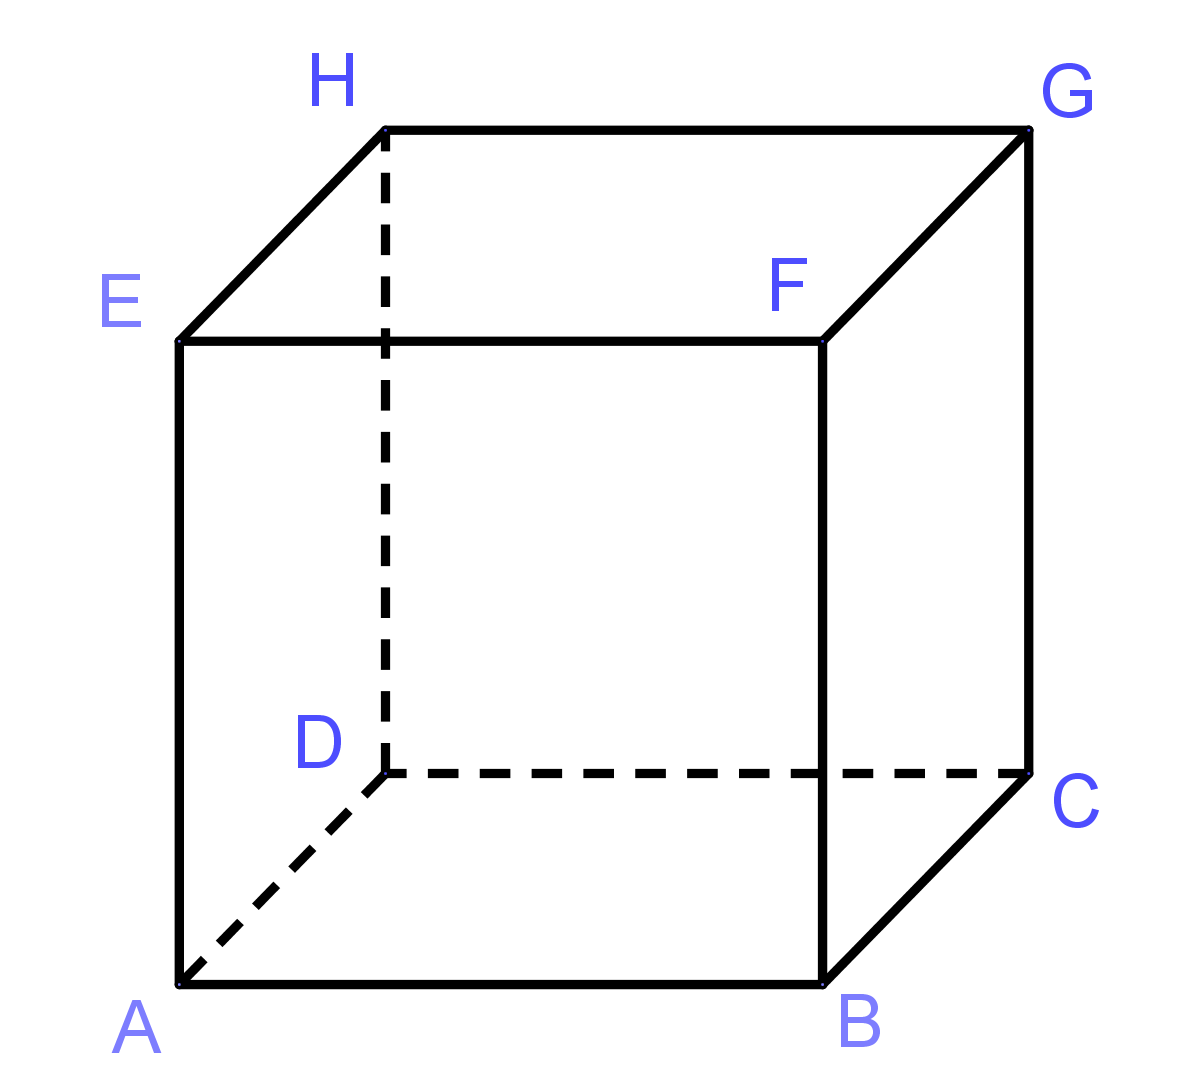
\includegraphics[scale=0.75]{cube}
\end{center}\end{minipage}\hfill \begin{minipage}{0.5\linewidth}

\begin{tabularx}{\linewidth}{XX}
$\overrightarrow{AD} \cdot \overrightarrow{AB}$ & $\overrightarrow{AD} \cdot \overrightarrow{FG}$ \\
$\overrightarrow{EH} \cdot \overrightarrow{ED}$ & $\overrightarrow{DH} \cdot \overrightarrow{FB}$\\
$\overrightarrow{CG} \cdot \overrightarrow{CE}$ & $\overrightarrow{EG} \cdot \overrightarrow{ED}$

\end{tabularx}

\end{minipage}

\end{exercise}

\begin{solution}On a ...
\begin{itemize}
\item $\overrightarrow{AD} \cdot \overrightarrow{AB} = AD \times AB \times \cos (\widehat{BAD})=1 \times 1 \times 0 = 0$
\item $\overrightarrow{AD} \cdot \overrightarrow{FG} = AD \times FG \times \cos(0)=1 \times 1 \times 1 = 1$ 
\item $\overrightarrow{EH} \cdot \overrightarrow{ED} = EH \times ED \times \cos(\widehat{HED})=1 \times \sqrt{2} \times \dfrac{\sqrt{2}}{2}=1$ 
\item $\overrightarrow{DH} \cdot \overrightarrow{FB} = DH \times FB \times \cos (180^{\circ})=1 \times 1 \times (-1) = -1$
\item $\overrightarrow{CG} \cdot \overrightarrow{CE} = CG \times CE \times \cos(\widehat{GCE})=1 \times \sqrt{3} \times \dfrac{1}{\sqrt{3}}=1$. On utilise ici la relation $\cos = \dfrac{\text{adjacent}}{\text{hypoténuse}}$ dans un triangle rectangle.
\item $\overrightarrow{EG} \cdot \overrightarrow{ED} = EG \times ED \times \cos(60^{\circ})=\sqrt{2} \times \sqrt{2} \times \sqrt{2} \times \dfrac{1}{2} = 1$

\end{itemize}\end{solution}




\begin{exercise}Est-il possible d'avoir 3 points de l'espace $A$, $B$ et $C$ tels que $AB=3$, $BC=6$ et $\overrightarrow{AB} \cdot \overrightarrow{AC} = 20$ ?\end{exercise}

\begin{solution}On aurait $\overrightarrow{AB}\cdot \overrightarrow{AC}=AB \times AC \times \cos(\widehat{BAC})$ et donc $\cos(\widehat{BAC})=\dfrac{\overrightarrow{AB}\cdot\overrightarrow{AC}}{AB \times AC}=\dfrac{20}{18}$. Un cosinus étant toujours entre $-1$ et $1$, c'est impossible.\end{solution}





\begin{exercise}Soit $\vec u$, $\vec v$ et $\vec w$ trois vecteurs tels que $\vec u \cdot \vec v = 3$, $\vec v \cdot \vec w=5$, $\vec u \cdot \vec w = -1$ et $\lvert \lvert \vec u \rvert \rvert=4$. 
\begin{enumerate}
\item Que vaut $ 2\vec u \cdot (3 \vec u - 2 \vec v + 4\vec w)$ ?
\item Que vaut $(3\vec v - 2 \vec u) \cdot (4\vec w + \vec u)$ ?
\end{enumerate}\end{exercise}

\begin{solution} $ 2\vec u \cdot (3 \vec u - 2 \vec v + 4\vec w)=6\lvert \lvert \vec u\rvert \rvert ^2-4\vec u \cdot \vec v + 8 \vec u \cdot \vec w = 96-12-8=76$

$(3\vec v - 2 \vec u) \cdot (4\vec w + \vec u)=12\vec v \cdot \vec w + 3 \vec v \cdot \vec u -8 \vec u \cdot \vec w -2 \lvert \lvert \vec u\rvert \rvert^2=60+9+8-32=45$
\end{solution}




\begin{exercise}On considère trois vecteurs $\vec u$, $\vec v$ et $\vec w$ tels que $\vec u \cdot \vec v = 3$ et $\vec u \cdot \vec w=4$. Montrer que le vecteur $\vec u$ est orthogonal au vecteur $4\vec v - 3 \vec w$.\end{exercise}

\begin{solution}On a alors $\vec u \cdot (4\vec v - 3 \vec w)=4\vec u \cdot \vec v -3\vec u \cdot \vec w = 12-12=0$

Le vecteur $\vec u$ est orthogonal au vecteur $4\vec v - 3 \vec w$.\end{solution}




\begin{exercise}Soit $\vec u$ et $\vec v$ deux vecteurs orthogonaux tels que $\lvert\lvert\vec{u}\rvert\rvert=3$ et $\lvert\lvert\vec{v}\rvert\rvert=7$. Que valent $\lvert\lvert\vec u + \vec v\rvert\rvert$ et $\lvert\lvert\vec u -\vec v\rvert\rvert$ ?\end{exercise}

\begin{solution}$\vec u$ et $\vec v$ sont orthogonaux, ce qui implique que $\vec u \cdot \vec v = 0$. On a 
\[\lvert\lvert\vec u + \vec v\rvert\rvert^2 = \lvert\lvert\vec{u}\rvert\rvert^2 + 2 \vec u \cdot \vec v + \lvert\lvert\vec{v}\rvert\rvert^2 = 3^2+2\times 0 + 7^2 = 58\]
et donc $\lvert\lvert\vec u + \vec v\rvert\rvert=\sqrt{58}$
\[\lvert\lvert\vec u - \vec v\rvert\rvert^2 = \lvert\lvert\vec{u}\rvert\rvert^2 - 2 \vec u \cdot \vec v + \lvert\lvert\vec{v}\rvert\rvert^2 = 3^2-2\times 0 + 7^2 = 58\]
et $\lvert\lvert\vec u - \vec v\rvert\rvert=\sqrt{58}$\end{solution}




\begin{exercise}Calculer $\vec{u} \cdot \vec{v}$ dans chacun des cas suivants.
\begin{enumerate}
\item $\lvert\lvert\vec{u}\rvert\rvert=2$, $\lvert\lvert\vec{v}\rvert\rvert=3$, $\lvert\lvert\vec{u}-\vec{v}\rvert\rvert=4$
\item $\lvert\lvert\vec{u}\rvert\rvert=5$, $\lvert\lvert\vec{v}\rvert\rvert=2$, $\lvert\lvert\vec{u}+\vec{v}\rvert\rvert=3$
\item $\lvert\lvert\vec{u}-\vec{v}\rvert\rvert=7$, $\lvert\lvert\vec{u}+\vec{v}\rvert\rvert=12$
\end{enumerate}\end{exercise}

\begin{solution} On a...
\begin{enumerate}
\item $\vec{u} \cdot \vec{v}= -\dfrac{1}{2}(\lvert\lvert\vec{u}-\vec{v}\rvert\rvert^2-\lvert\lvert\vec{u}\rvert\rvert^2-\lvert\lvert\vec{v}\rvert\rvert^2)=-\dfrac{1}{2}(4^2-3^2-2^2)=\dfrac{3}{2}$
\vskip5pt
\item $\vec{u} \cdot \vec{v}= \dfrac{1}{2}(\lvert\lvert\vec{u}+\vec{v}\rvert\rvert^2-\lvert\lvert\vec{u}\rvert\rvert^2-\lvert\lvert\vec{v}\rvert\rvert^2)=\dfrac{1}{2}(3^2-5^2-2^2)=-10$
\vskip5pt
\item $\vec{u} \cdot \vec{v} = \dfrac{1}{4}( \lvert\lvert\vec{u}+\vec{v}\rvert\rvert^2-\lvert\lvert\vec{u}-\vec{v}\rvert\rvert^2 )=\dfrac{1}{4}(12^2-7^2)=\dfrac{95}{4}$
\end{enumerate}\end{solution}



\begin{exercise}Soit $\vec u$ et $\vec v$ deux vecteurs tels que $\lvert\lvert\vec{u}\rvert\rvert=3$, $\lvert\lvert\vec{v}\rvert\rvert=4$ et $\lvert\lvert\vec{u-v}\rvert\rvert=5$. Montrer que $\vec u$ et $\vec v$ sont orthogonaux.\end{exercise}

\begin{solution}$\vec u \cdot \vec v = -\dfrac{1}{2}(\lvert\lvert\vec{u}-\vec{v}\rvert\rvert^2-\lvert\lvert\vec{u}\rvert\rvert^2-\lvert\lvert\vec{v}\rvert\rvert^2)=-\dfrac{1}{2}(5^2-3^2-4^2)=-\dfrac{1}{2}(25-9-16)=0$. $\vec u$ et $\vec v$ sont orthogonaux.\end{solution}




\begin{exercise}Soit $A$, $B$ et $C$ trois points de l'espace tel que $AB+BC=AC$. Montrer que ces points sont alignés.\end{exercise}

\begin{solution}On a alors $BA + BC = AC$. Or, $\overrightarrow{BA}-\overrightarrow{BC}=\overrightarrow{BA}+\overrightarrow{CB}=\overrightarrow{CA}$. Utilisons alors les formules de polarisation.

On a $\overrightarrow{BA}\cdot\overrightarrow{BC}=-\dfrac{1}{2}(\lvert\lvert\overrightarrow{BA}-\overrightarrow{BC}\rvert\rvert^2-AB^2-BC^2)=-\dfrac{1}{2}(CA^2-AB^2-BC^2)$. En remplaçant $CA$ par $BA+BC$, on a alors $\overrightarrow{BA} \cdot \overrightarrow{BC} = -\dfrac{1}{2}((BA+BC)^2-AB^2-BC^2)=-\dfrac{1}{2}(BA^2+2BA \times BC+BC^2-AB^2-BC^2)=BA \times BC$.

Or, $\overrightarrow{BA} \cdot \overrightarrow{BC} = AB \times BC \times \cos (\widehat{ABC})$. Il en vient que $\cos (\widehat{ABC})=-1$ et que l'angle entre les vecteurs $\widehat{ABC}$ mesure donc 180 degrés. Cela signifie que les points $A$, $B$ et $C$ sont alignés (et même que le point $B$ se situe entre $A$ et $C$).\end{solution}


\section*{Base orthonormée}



\begin{exercise}L'espace est muni d'un repère $\Oijk$ orthonormé. Montrer que \coorde{u}{1}{5}{-9} et \coorde{v}{3}{3}{2} sont orthogonaux.\end{exercise}

\begin{solution}On a $\vec u \cdot \vec v = 1 \times 3 + 5 \times 3 - 9 \times 2 =0$. $\vec u$ et $\vec v$ sont orthogonaux.\end{solution}



\begin{exercise}L'espace est muni d'un repère $\Oijk$ orthonormé. Soit $x$ un réel. On considère les points $A(2;5;1)$, $B(3;1;2)$, $C(8;2;x)$. 

\begin{enumerate}
\item Déterminer les coordonnées des vecteurs $\overrightarrow{AB}$ et $\overrightarrow{AC}$
\item Pour quelle valeur du réel $x$ les vecteurs $\overrightarrow{AB}$ et $\overrightarrow{AC}$ sont-ils orthogonaux ?
\end{enumerate}
\end{exercise}

\begin{solution} \coorde{AB}{1}{-4}{1} et \coorde{AC}{6}{-3}{x-1}. $\overrightarrow{AB}$ et $\overrightarrow{AC}$ sont orthogonaux si et seulement si $\overrightarrow{AB}\cdot \overrightarrow{AC}=0$, c'est-à-dire $1 \times 6 -4 \times (-3) + 1 \times (x-1)=0$ c'est-à-dire $19+x=0$ d'où $x=-17$\end{solution}




\begin{exercise}L'espace est muni d'un repère $\Oijk$ orthonormé. Soit $x$ un réel. On considère les points $A(3;4;2)$, $B(5;2;2x)$, $C(3;10;x)$. Pour quelles valeurs du réel $x$ les vecteurs $\overrightarrow{AB}$ et $\overrightarrow{AC}$ sont-ils orthogonaux ?\end{exercise}

\begin{solution}On a \coorde{AB}{2}{-2}{2x-2} et \coorde{AC}{0}{6}{x-2}. $\overrightarrow{AB}$ et $\overrightarrow{AC}$ sont orthogonaux si et seulement si $\overrightarrow{AB}\cdot \overrightarrow{AC}=0$, c'est-à-dire $2 \times 0 -2\times 6 +(2x-2) \times (x-2)=0$

On a donc $2x^2-6x-8=0$. C'est un polynôme du second degré dont les racines sont $-1$ et $4$. $\overrightarrow{AB}$ et $\overrightarrow{AC}$ sont orthogonaux si et seulement si $x=-1$ ou $x=4$\end{solution}





\begin{exercise}L'espace est muni d'un repère $\Oijk$ orthonormé. On considère les points $A(-1;2;0)$, $B(1;2;4)$, $C(-1;1;1)$.
\begin{enumerate}
\item Montrer que les points $A$, $B$ et $C$ ne sont pas alignés.
\item Calculer $\overrightarrow{AB}\cdot \overrightarrow{AC}$
\item Calculer les longueurs $AB$ et $AC$.
\item En déduire une mesure de l'angle $\widehat{BAC}$ arrondie eu degré près.
\end{enumerate}\end{exercise}

\begin{solution}On a $\coorde{AB}{1-(-1)}{2-2}{4-0}=\coordbe{2}{0}{4}$ et $\coorde{AC}{-1-(-1)}{1-2}{1-0}=\coordbe{0}{-1}{1}$. Les vecteurs $\overrightarrow{AB}$ et $\overrightarrow{AC}$ ne sont pas colinéaires, les points $A$, $B$ et $C$ ne sont pas alignés.

Puisque l'on est dans un repère orthonormé, $\overrightarrow{AB}\cdot \overrightarrow{AC}=2 \times 0+0 \times -1 + 4 \times 1 = 4$.

On a $AB = \sqrt{2^2+0^2+4^2}=\sqrt{20}$ et $BC=\sqrt{0^2+(-1)^2+1^2}=\sqrt{2}$.

On sait  que $4=\overrightarrow{AB}\cdot \overrightarrow{AC}=AB \times AC \times \cos (\widehat{BAC})$. 

Ainsi, $\sqrt{20} \times \sqrt{2} \times \cos (\widehat{BAC}) = 4$ d'où $\cos (\widehat{BAC})=\dfrac{2}{\sqrt{10}}$ et l'angle $\widehat{BAC}$ mesure environ 51 degrés (utiliser arccos ou cos$^{-1}$ sur la calculatrice).\end{solution}





\begin{exercise}
On considère un cube $ABCDEFGH$ d'arêtes de longueur 1 ainsi que les points $I$, $J$ et $K$, centres respectifs des faces $ABCD$, $BCGF$ et $ABFE$. On se place dans le repère orthonormé $(A;\overrightarrow{AB},\overrightarrow{AD},\overrightarrow{AE})$.

\begin{minipage}{0.4\linewidth}
\begin{center}
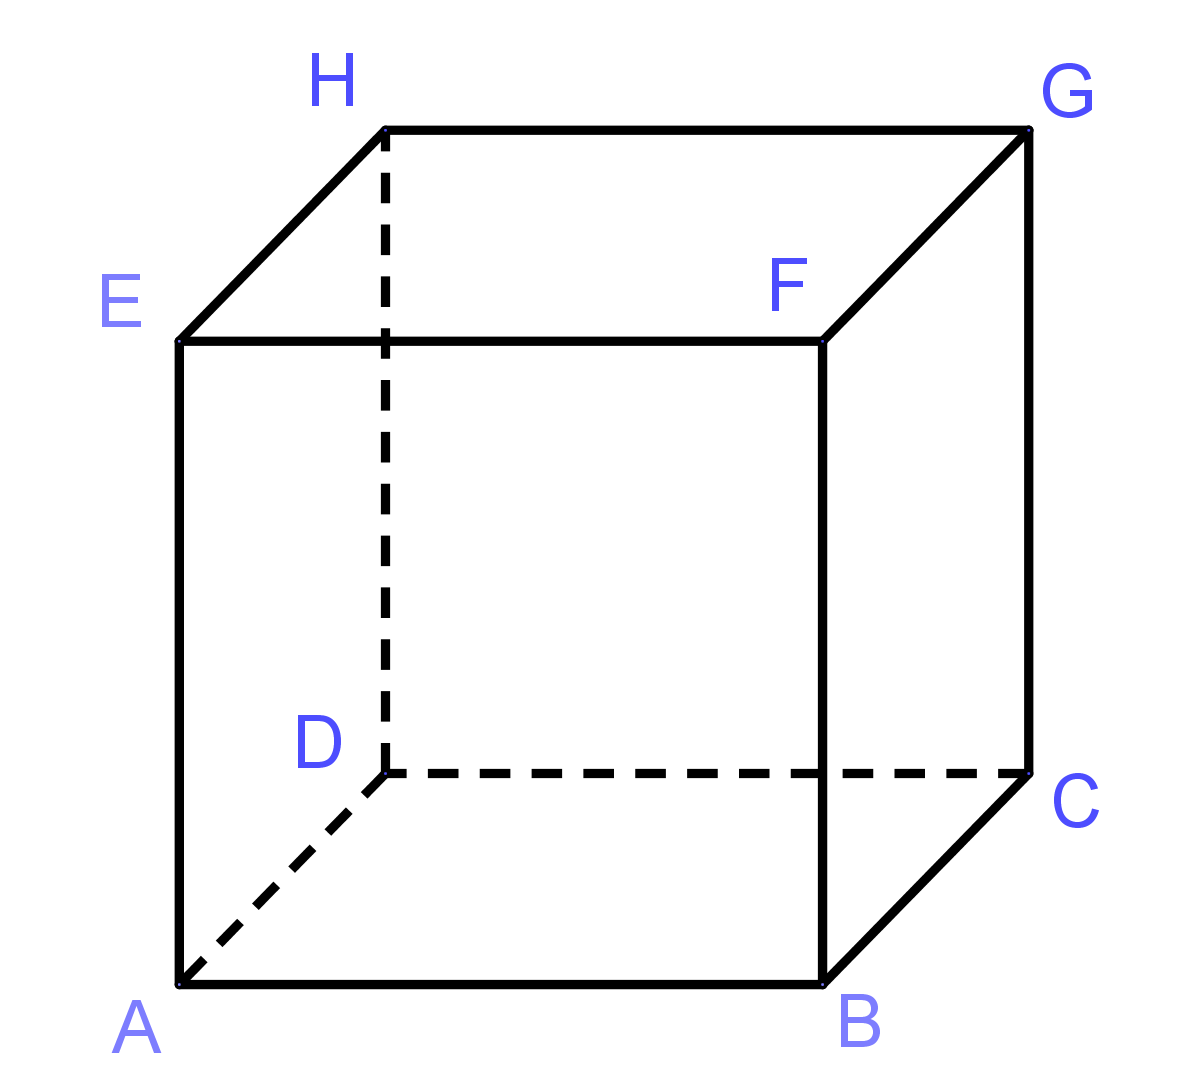
\includegraphics[scale=0.8]{cube}
\end{center}\end{minipage}\hfill \begin{minipage}{0.5\linewidth}
\begin{enumerate}
\item Donner les coordonnées des points $I$, $J$ et $K$ dans ce repère.
\item Calculer $\overrightarrow{IJ} \cdot \overrightarrow{IK}$
\item En déduire la valeur de l'angle $\widehat{JIK}$.
\item Quelle est la nature du triangle $IJK$ ?
\end{enumerate}
\end{minipage}

\end{exercise}

\begin{solution}Les points $I$, $J$ et $K$  ont pour coordonnées $\left( \dfrac{1}{2};\dfrac{1}{2};0\right)$, $\left(1;\dfrac{1}{2};\dfrac{1}{2}\right)$ et $\left( \dfrac{1}{2} ; 0;\dfrac{1}{2}\right)$ comme coordonnées respectives dans le repère $(A;\overrightarrow{AB},\overrightarrow{AD},\overrightarrow{AE})$.

On a \coorde{IJ}{0.5}{0}{0.5} et \coorde{IK}{0}{-0.5}{0.5}. Puisque le repère $(A;\overrightarrow{AB},\overrightarrow{AD},\overrightarrow{AE})$ est orthonormé,
\[ \overrightarrow{IJ}\cdot \overrightarrow{IK}=0.5 \times 0 - 0 \times 0.5 + 0.5 \times 0.5 = 0.25 = \dfrac{1}{4} \]

On sait de plus que $\overrightarrow{IJ} \cdot \overrightarrow{IK}=IJ \times IK \times \cos (\widehat{JIK})$. Or,
\begin{itemize}
\item $IJ=\sqrt{0.5^2+0^2+0.5^2}=\sqrt{0.5}=\dfrac{\sqrt{2}}{2}$
\item $IK=\sqrt{0^2+(-0.5)^2+0.5^2}=\sqrt{0.5}=\dfrac{\sqrt{2}}{2}$
\end{itemize}
Ainsi, $\cos (\widehat{JIK})=\dfrac{\frac{1}{4}}{\frac{\sqrt{2}}{2}\times \frac{\sqrt{2}}{2}}=\dfrac{1}{2}$ et donc $\widehat{JIK}=\dfrac{\pi}{3}$.

 Puisque $IJ=IK$, le triangle $IJK$ est isocèle en $I$. On a donc  $\widehat{JKI}=\widehat{IJK}$. Or, $\widehat{JIK}=\dfrac{\pi}{3}$ et la somme des angles d'un triangle vaut $\pi$ radians. On a donc $\widehat{JKI}=\widehat{IJK}=\dfrac{\pi}{3}$. Le triangle $IJK$ est donc équilatéral.\end{solution}
 
\begin{exercise}On se place dans un repère orthonormé $\Oijk$. On considère les vecteurs $\coorde{u}{1}{0}{1}$, $\coorde{v}{0}{1}{1}$ et $\coorde{w}{1}{1}{0}$.
\begin{enumerate}
\item Montrer que les vecteurs $\vec u$, $\vec v$ et $\vec w$ ne sont pas coplanaires.
\item Soit $\lambda$ un réel et $\vec V = \vec v + \lambda \vec u$. Déterminer la valeur de $\lambda$ pour que $\vec V$ et $\vec u$ soient orthogonaux.
\item Soit $\mu_1$ et $\mu_2$ deux réels et $\vec W = \vec w + \mu_1 \vec V + \mu_2 \vec u$. Déterminer les valeurs de $\mu_1$ et $\mu_2$ pour que le vecteur $\vec W$ soit orthogonal aux vecteurs $\vec V$ et $\vec u$.
\item En déduire une base orthonormée de l'espace différente de $(\vec{\imath}\, ;\, \vec{\CMjmath} \,;\, \vec k)$.
\end{enumerate}
Ce procédé pour exhiber une base orthonormée à partir de vecteurs non coplanaires est appelé algorithme de Gram-Schmidt.\end{exercise}

\begin{solution}\hspace{0pt}

\begin{enumerate}
\item Les vecteurs $\vec v$ et $\vec w$ ne sont pas colinéaires. Sont donc $a$ et $b$ des réels tels que $\vec u=a\vec v+b\vec w$.

On a alors \coordbe{1}{0}{1} = \coordbe{b}{a+b}{a}, ce qui est impossible. Les vecteurs $\vec u$, $\vec v$ et $\vec w$ ne sont donc pas coplanaires.

\item On souhaite que $\vec V$ et $\vec u$ soient orthogonaux. On a donc $\vec V \cdot \vec u = 0$. Or, $\vec V \cdot \vec u =(\vec v + \lambda \vec u) \cdot \vec u = \vec v \cdot \vec u + \lambda \vec u \cdot \vec u$.

De plus, $\vec v \cdot \vec u = 1$ et $\vec u \cdot \vec u =2$. Ainsi, $\vec V \cdot \vec u = 0$ si et seulement si $1+2\lambda = 0$ soit $\lambda = -\dfrac{1}{2}$. On considère donc $\vec V = \vec v - \dfrac{1}{2}\vec u$. Le vecteur $\vec V$ a pour coordonnées \coordbe{-1/2}{1}{1/2}.

\item On souhaite que $\vec W$ et $\vec V$ soient orthogonaux. On a donc $\vec W \cdot \vec V = 0$. Or, $\vec W \cdot \vec V =(\vec w + \mu_1 \vec V + \mu_2 \vec u) \cdot \vec V = \vec w \cdot \vec V + \mu_1 \vec V \cdot \vec V + \mu_2 \vec u \cdot \vec V$.

De plus, $\vec w \cdot \vec V = \dfrac{1}{2}$, $\vec V \cdot \vec V = \dfrac{3}{2}$ et $\vec u \cdot \vec V =0$. Ainsi, $\vec W \cdot \vec V = 0$ si et seulement si $\dfrac{1}{2}+\dfrac{3}{2}\mu_1 = 0$ soit $\mu_1 = -\dfrac{1}{3}$. 

On souhaite que $\vec W$ et $\vec u$ soient orthogonaux. On a donc $\vec W \cdot \vec u = 0$. Or, $\vec W \cdot \vec u =(\vec w + \mu_1 \vec V + \mu_2 \vec u) \cdot \vec u = \vec w \cdot \vec u + \mu_1 \vec V \cdot \vec u + \mu_2 \vec u \cdot \vec u$.

De plus, $\vec w \cdot \vec u = 1$, $\vec V \cdot \vec u = 0$ et $\vec u \cdot \vec u =2$. Ainsi, $\vec W \cdot \vec u = 0$ si et seulement si $1+2\mu_2 = 0$ soit $\mu_2 = -\dfrac{1}{2}$. 

On considère donc $\vec W = \vec w - \dfrac{1}{3}\vec V - \dfrac{1}{2}\vec u$. Le vecteur $\vec W$ a pour coordonnées \coordbe{2/3}{2/3}{-2/3}.

\item Les vecteurs $\vec u$, $\vec V$ et $\vec W$ forment une base orthogonale de l'espace. Pour avoir une base orthonormé, il suffit de diviser chacun de ces vecteurs par sa norme.
 \end{enumerate}\end{solution}
 


\section*{Orthogonalité}

\begin{exercise}On se place dans un repère orthonormé $\Oijk$. On considère les points $A(2;5;1)$, $B(3;2;3)$ et $C(3;6;2)$.
\begin{enumerate}
\item Calculer les coordonnées des vecteurs $\overrightarrow{AB}$ et $\overrightarrow{AC}$.
\item Montrer que les droites $(AB)$ et $(AC)$ sont perpendiculaires.
\end{enumerate}\end{exercise}

\begin{solution}On a \coorde{AB}{1}{-3}{2} et \coorde{AC}{1}{1}{1}

$\overrightarrow{AB} \cdot \overrightarrow{AC}= 1\times 1 -3 \times 1 +2 \times 1 =0$. Les vecteurs $\overrightarrow{AB}$ et $\overrightarrow{AC}$ sont orthogonaux. Les droites $(AB)$ et $(AC)$ sont donc orthogonales. De plus, ces droites ont le point $A$ en commun, elles sont donc perpendiculaires.\end{solution}

%

\begin{exercise}On se place dans un cube $ABCDEFGH$.
\begin{enumerate}
\item Quelle est la nature du repère $(A;\overrightarrow{AB},\overrightarrow{AD},\overrightarrow{AE})$ ?
\item Déterminer les coordonnées des points $F$, $D$, $B$ et $H$ dans ce repère.
\item En déduire les coordonnées des vecteurs $\overrightarrow{DF}$ et $\overrightarrow{BH}$.
\item Les droites $(DF)$ et $(BH)$ sont-elles perpendiculaires ?
\end{enumerate}\end{exercise}

\begin{solution}Ce repère est orthonormé.

On a $F(1,0,1)$, $D(0,1,0)$, $B(1,0,0)$, $H(0,1,1)$, \coorde{DF}{-1}{1}{-1} et \coorde{BH}{-1}{1}{1}.

 $\overrightarrow{DF}\cdot \overrightarrow{BH}=-1\times (-1) + 1 \times 1 -1\times 1 = 1 \neq 0$. Les droite $(DF)$ et $(BH)$ ne sont pas perpendiculaires.\end{solution}
 
 

\begin{exercise}On considère les points $A(2;1;5)$ et $B(3;2;3)$ ainsi que la droite $\Delta$ admettant pour représentation paramétrique \[ \Delta : \left\{\renewcommand{\arraystretch}{1}\renewcommand{\arraystretch}{1}\begin{array}{l} x = 4 +3t \\ y = 2+t \\ z = -5+2t 

\end{array}\right. , t\in \mathbb{R}.\] Les droites $(AB)$ et $\Delta$ sont-elles orthogonales ?\end{exercise}

\begin{solution}La droite $\Delta$ est dirigée par le vecteur \coorde{u}{3}{1}{2}. La droite $(AB)$ est dirigée par le vecteur \coorde{AB}{1}{-1}{-2}. Par ailleurs, $\overrightarrow{AB}\cdot \vec u = 1 \times 3 - 1 \times 1  -2 \times 2 = 0$. Les droites $(AB)$ et $\Delta$ sont orthogonales.\end{solution}


\begin{exercise}L'espace est muni d'un repère $\Oijk$ orthonormé. On considère deux droites $(d_1)$ et $(d_2)$ admettant pour représentations paramétriques respectives

\[ (d_1) : \left\{ \renewcommand{\arraystretch}{1}\renewcommand{\arraystretch}{1}\begin{array}{l}x=2+t \\ y=3-t \\ z=t \end{array}\right.,t \in \mathbb{R} \quad \text{et} (d_2) : \left\{ \renewcommand{\arraystretch}{1}\renewcommand{\arraystretch}{1}\begin{array}{l}x=-5+2t' \\ y=-1+t' \\ z=5 \end{array}\right.,t' \in \mathbb{R}.\]

\begin{enumerate}
\item Donner un vecteur directeur $\vec u_1$ de la droite $(d_1)$ et un vecteur directeur $\vec u_2$ de la droite $(d_2)$.
\item Montrer que le vecteur $\coorde{v}{1}{-2}{-3}$ est orthogonal à $\vec u_1$ et à $\vec u_2$.
\item Montrer que le point $B(3;3;5)$ appartient à la droite $(d_2)$.
\item Montrer que la droite $\Delta$ passant par le point $B$ et dirigé par le vecteur $\vec v$ est perpendiculaire aux droites $(d_1)$ et $(d_2)$.
\end{enumerate}\end{exercise}

\begin{solution}\hspace{0pt}
\begin{enumerate}
\item Le vecteur \coorde{u_1}{1}{-1}{1} dirige la droite $(d_1)$. Le vecteur \coorde{u_2}{2}{1}{0} dirige la droite $(d_2)$.
\item On considère le vecteur $\coorde{v}{1}{-2}{-3}$ .

\begin{itemize}
\item $\vec v \cdot \vec u_1 = 1 \times 1 - 2 \times (-1) -3 \times 1 =0$ ;
\item $\vec v \cdot \vec u_2 = 1 \times 2 -2 \times 1 -3 \times 0 =0$.
\end{itemize}

$\vec v$ est orthogonal à $\vec u_1$ et à $\vec u_2$.
\item En prenant $t'=4$ dans l'équation de $(d_2)$, on obtient le point de coordonnées $(3;3;5)$. Le point $B(3;3;5)$ appartient à la droite $(d_2)$
\item La droite $\Delta$ passant par le point $B$ et dirigé par le vecteur $\vec v$ est perpendiculaire à la droite $(d_2)$. En effet $\vec v$ et $\vec u_2$ sont orthogonaux et les deux droites ont en commun le point $B$.
On sait de plus que $(d_1)$ et $\Delta$ sont orthogonales. Il reste à montrer qu'elles sont sécantes. 

Une représentation paramétrique de $\Delta$ est $\left\{ \renewcommand{\arraystretch}{1}\renewcommand{\arraystretch}{1}\begin{array}{l}x=3+t' \\ y=3-2t' \\ z=5-3t' \end{array}\right.,t' \in \mathbb{R}.$

Chercher l'intersection de $(d_1)$ et $\Delta$ revient à chercher deux réels $t$ et $t'$ tels que $\coordbe{2+t}{3-t}{t}=\coordbe{3+t'}{3-2t'}{5-3t'}$.

La dernière ligne permet d'exprimer $t$ en fonction de $t'$. remplaçons $t$ par $5-3t'$ dans la première ligne. On obtient alors $2+5-3t'=3+t'$ d'où $t'=1$. Puisque $t=5-3t'$, on a alors $t=2$.

Vérifions : en remplaçant $t$ par $2$ dans l'équation de $(d_1)$, on obtient le point de coordonnées $(4;1;;2)$. En replaçant $t'$ par 1 dans l'équation de $\Delta$, on obtient le point de coordonnées $(4;1;2)$. Les droites $\Delta$ et $(d_1)$ sont donc sécantes. Puisqu'elles sont orthogonales, elles sont donc perpendiculaires.

Ainsi, $\Delta$ est perpendiculaire à $(d_1)$ et $(d_2)$.
\end{enumerate}\end{solution}



\begin{exercise}L'espace est muni d'un repère $\Oijk$ orthonormé. On considère les points $A(1;2;1)$, $B(3;4;1)$, $C(4;-1;6)$ et $D(6;1;6)$. Montrer que $ABDC$ est un rectangle.\end{exercise}

\begin{solution}D'une part, on a \coorde{AB}{3-1}{4-2}{1-1} soit \coorde{AB}{2}{2}{0} et \coorde{CD}{6-4}{1-(-1)}{6-6} soit \coorde{CD}{2}{2}{0}. Ainsi, $\overrightarrow{AB}=\overrightarrow{CD}$. Les points $A$, $B$, $C$ et $D$ sont donc coplanaires et $ABDC$ est un parallélogramme.

De plus, on a \coorde{BD}{6-3}{1-4}{6-1} soit \coorde{BD}{3}{-3}{5}.

Ainsi, $\overrightarrow{AB} \cdot \overrightarrow{BD} = 2 \times 3 - 2 \times 3 + 0 \times 5 = 0$. L'angle $\widehat{ABD}$ est un angle droit. $ABDC$ est un parallélogramme ayant un angle droit, c'est donc un rectangle.\end{solution}




\begin{exercise}On se place dans un repère orthonormé $\Oijk$. Soit \coorde{v_1}{1}{4}{1}, \coorde{v_2}{3}{2}{-2} et \coorde{u}{2}{-1}{2}.

On considère le plan $\mathcal{P}$ passant par $O$ et dirigé par les vecteurs $\vec v_1$ et $\vec v_2$.  Montrer que le vecteur $\vec u$ est normal au plan $\mathcal{P}$.\end{exercise}

\begin{solution}Puisque le repère  $\Oijk$ est orthonormé, on a donc
\begin{itemize}
\item $\vec v_1 \cdot \vec u = 1 \times 2 + 4 \times (-1)+ 1\times 2=0$ ;
\item $\vec v_2 \cdot \vec u = 3 \times 2 - 1 \times 1 -2 \times 2 =0$.
\end{itemize}
Ainsi, $\vec u$ est orthogonal à $\vec v_1$ et $\vec v_2$ qui sont deux vecteurs non colinéaires du plan $\mathcal{P}$. $\vec u$ est normal au plan $P$.\end{solution}



\begin{exercise}
 L'espace est muni d'un repère $(O;\vec{\imath}; \vec{\CMjmath}; \vec k)$ orthonormé. On considère les points $A(3;-2;-2)$, $B(1;3;-8)$ et $C(-2;0;4)$ ainsi que le vecteur \coorde{n}{2}{2}{1}. Montrer que $\vec n$ est un vecteur normal au plan $(ABC)$.
\end{exercise}

\begin{solution}On a 
 \begin{itemize}
 \item $\vec n \cdot \overrightarrow{AB} = 2 \times (1-3) + 2 \times (3-(-2))+1 \times (-8-(-2)) = 0$ ;
 \item $\vec n \cdot \overrightarrow{AC} = 2 \times (-2-3) + 2 \times (0-(-2))+1 \times (4-(-2)) = 0$.
 \end{itemize}
 
 Ainsi, $\vec n$ est orthogonal aux vecteurs $\overrightarrow{AB}$ et $\overrightarrow{AC}$. Il est donc normal au plan $(ABC)$.
 \end{solution} 
 
 
 \begin{exercise}L'espace est muni d'un repère $(O;\vec{\imath}; \vec{\CMjmath}; \vec k)$ orthonormé. On considère les points $A(1;3;-1)$, $B(2;4;1)$ et $C(0;1;1)$.
 \begin{enumerate}
 \item Justifier que les points $A$, $B$ et $C$ forment bien un plan.
 \item Déterminer un vecteur normal au plan $(ABC)$.
 \end{enumerate}\end{exercise}
 
\begin{solution}
On a \coorde{AB}{1}{1}{2} et \coord{AC}{-1}{-2}{2}. Les vecteurs $\overrightarrow{AB}$ et $\overrightarrow{AC}$ ne sont pas colinéaires. Les points $A$, $B$ et $C$ ne sont donc pas alignés et forment donc un plan.

Soit \coorde{n}{x}{y}{z} un vecteur normal au plan $(ABC)$.

On a alors $\vec n \cdot \overrightarrow{AB}=0$ et donc $x+y+2z=0$. Ainsi, on a $x=-y-2z$.

On a également $\vec n \cdot \overrightarrow{AC}=0$ et donc $-x-2y+2z=0$. En remplaçant $x$ par $-y-2z$, on trouve alors $y+2z-2y+2z=0$ et donc $-y+4z=0$ soit $y=4z$.

Prenons alors $z=1$. On a alors $y=4$ et $x=-4-2=-6$. On peut alors vérifier que le vecteur \coorde{n}{-6}{4}{1} est normal au plan $(ABC)$.
\end{solution} 




\section*{Equations cartésiennes de plan}

Dans tous les exercices suivants, l'espace est muni d'un repère $\Oijk$ orthonormé.

\begin{exercise}On considère le plan $\mathcal{P}$ d'équation $3x+2y-z+1=0$ ainsi que les points $A(2,-3,1)$, $B(0,0,1)$, $C(0,2,5)$ et $D(1,5,3)$.
\begin{enumerate}
\item Quels sont les points qui appartiennent au plan $\mathcal{P}$ ?
\item Les points $A$, $B$, $C$ et $D$ sont-ils coplanaires ?
\end{enumerate}\end{exercise}

\begin{solution}On regarde quels sont les points dont les coordonnées vérifient l'équation de $\mathcal{P}$. Pour le point $A$, on a $3 \times 2 +2 \times(-3)-1+1=0$, le point $A$ appartient au plan $\mathcal{P}$. De même, les points $B$ et $C$ appartiennent à ce plan. En revanche, $3 \times 1 +2 \times 5-3+1=11 \neq 0$. Le point $D$ n'appartient donc pas au plan $\mathcal{P}$.

On a \coorde{AB}{-2}{3}{0} et \coorde{AC}{-2}{5}{4}. Les vecteurs $\overrightarrow{AB}$ et $ \overrightarrow{AC}$ ne sont pas colinéaires, les point $A$, $B$ et $C$ ne sont donc pas alignés. Ils définissent bien un plan $(ABC)$ qui n'est autre que le plan $\mathcal{P}$. Or, $D$ n'appartient pas à ce plan, les points $A$, $B$, $C$ et $D$ ne sont donc pas coplanaires.
\end{solution}



\begin{exercise}Soit $P$ le plan d'équation $2x-5y+3z-2=0$ et $(d)$ la droite de représentation paramétrique $\left\{\renewcommand{\arraystretch}{1}\renewcommand{\arraystretch}{1}\begin{array}{l}x=2-2t \\ y=1+t \\z=1+3t\end{array}\right.$. Montrer que la droite $(d)$ est incluse dans le plan $P$.\end{exercise}

\begin{solution}Pour tout réel $t$, $2(2-2t)-5(1+t)+3(1+3t)-2=4-4t-5-5t+3+9t-2=0$. Tous les points de la droite $(d)$ appartiennent donc au plan $P$.\end{solution}



\begin{exercise}Donner une équation cartésienne du plan passant par le point $A(2;5;-1)$ et de vecteur normal \coorde{n}{2}{-3}{1}\end{exercise}

\begin{solution}Une équation cartésienne du plan passant par le point $A(2;5;-1)$ et de vecteur normal \coorde{n}{2}{-3}{1} est \\ $ 2(x-2)-3(y-5)+(z+1)=0$ c'est-à-dire $2x-3y+z+12=0$.\end{solution}



\begin{exercise} On considère les points $A(-1;2;0)$, $B(1;2;4)$, $C(-1;1;1)$, $D(5;3;0)$.

\begin{enumerate}
\item Montrer que le vecteur \coorde{n}{2}{-1}{-1} est normal au plan $(ABC)$.
\item Donner une équation cartésienne du plan $(ABC)$.
\item Le point $D$ appartient-il à ce plan ?
\item Donner une équation cartésienne du plan parallèle au plan $(ABC)$ passant par $D$.
\end{enumerate}\end{exercise}

\begin{solution}On a \coorde{AB}{2}{0}{4} et \coorde{AC}{0}{-1}{1}. Ainsi,
\begin{itemize}
\item $\vec n \cdot \overrightarrow{AB}=2\times 2 +(-1) \times 0 + (-1) \times 4 = 0$ ;
\item $\vec n \cdot \overrightarrow{AC}=2\times 0 + (-1) \times (-1) + (-1) \times 1 = 0$.
\end{itemize}
Ainsi, le vecteur \coorde{n}{2}{-1}{-1} est normal eu plan $(ABC)$.

Le plan $(ABC)$ passe par $A$ et admet le vecteur $\vec n$ comme vecteur normal. Une équation cartésienne du plan $(ABC)$ est donc $2(x-(-1))-1(y-2)-1(z-0)$, c'est-à-dire $2x-y-z+4=0$.

Le plan parallèle au plan $(ABC)$ passant par $D$ admet également le vecteur $\vec n$ comme vecteur normal. Une équation de ce plan est donc $2(x-5)-(y-3)-(z-0)=0$
c'est-à-dire $2x-y-z-7=0$.\end{solution}



\begin{exercise}Soit $P_1$ et $P_2$ les plans d'équations cartésiennes respectives $2x+3y-5z+1=0$ et $4x+6y-10z+3=0$. Montrer que les plans $P_1$ et $P_2$ sont parallèles mais non confondus.\end{exercise}

\begin{solution}Les vecteurs \coorde{u}{2}{3}{-5} et \coorde{v}{4}{6}{-10} sont normaux respectivement aux plans $P_1$ et $P_2$. Ces vecteurs sont colinéaires, les plans $P_1$ et $P_2$ sont donc parallèles.\end{solution}



\begin{exercise}On considère les points $A(2;-1;0)$, $B(1;0;-3)$ et $C(6;6;1)$ ainsi que le plan $\mathcal{P}$ d'équation  $2x-y-z+4=0$. Montrer que le plan $\mathcal{P}$ est parallèle au plan $(ABC)$.\end{exercise}

\begin{solution}Le vecteur \coorde{u}{2}{-1}{-1} est normal au plan $\mathcal{P}$. De plus,
\begin{itemize}
\item $\vec u \cdot \overrightarrow{AB} = 2(1-2)-(0-(-1))-(-3-0)=-2-1-3=0$ ;
\item $\vec u \cdot \overrightarrow{AC} = 2(6-2)-(6-(-1))-(1-0)=8-7-1=0$.
\end{itemize}
Le vecteur $\vec u$ est donc également normal au plan $(ABC)$. Les plans $\mathcal{P}$ et $(ABC)$ sont donc parallèles.\end{solution}





\begin{exercise}Déterminer, s'il existe, les coordonnées du point d'intersection du plan $P$ d'équation  $ 2x-3y-2z+1=0$ et de la droite $(d)$ de représentation paramétrique $\left\{ \renewcommand{\arraystretch}{1}\renewcommand{\arraystretch}{1}\begin{array}{l}x=1+t \\ y=1+2t \\ z = 5-3t \\\end{array}\right., t \in \mathbb{R}$.\end{exercise}

\begin{solution}Supposons qu'il existe un point $M(x;y;z)$ dans $P \cap (d)$. On a alors $\left\{ \renewcommand{\arraystretch}{1}\renewcommand{\arraystretch}{1}\begin{array}{l}x=1+t \\ y=1+2t \\ z = 5-3t \\ 2x-3y-2z+1=0 \end{array}\right.$.

En remplaçant les $x$, $y$ et $z$ de la dernière ligne, on obtient. $2(1+t)-3(1+2t)-2(5-3t)+1=0$ c'est-à-dire $t=5$. Vérifions : en remplaçant $t$ par 5 dans l'équation de $(d)$, on obtient le point de coordonnées $(6;11;-10)$. Or, $2\times 6 -3 \times 11 -2 \times (-10)+1=0$. Ce point appartient également au plan $P$.\end{solution}




\begin{exercise}On considère les plans $\mathcal{P}_1$ et $\mathcal{P}_2$ d'équations respectives $2x+y-z+3=0$ et $3x+2y-z+1=0$.

\begin{enumerate}
\item Donner un vecteur normal à $\mathcal{P}_1$ et un vecteur normal à $\mathcal{P}_2$. Ces plans sont-ils parallèles ?
\item Montrer que les points $A(1;1;6)$ et $B(2;0;7)$ appartiennent aux plans $\mathcal{P}_1$ et $\mathcal{P}_2$.
\item En déduire une représentation paramétrique de $\mathcal{P}_1 \cap \mathcal{P}_2$.
\end{enumerate}\end{exercise}

\begin{solution}Un vecteur normal à $\mathcal{P}_1$ est le vecteur \coorde{u_1}{2}{1}{-1}. Un vecteur normal à $\mathcal{P}_2$ est le vecteur \coorde{u_2}{3}{2}{-1}. Ces vecteurs ne sont pas colinéaires. Les plans $\mathcal{P}_1$ et $\mathcal{P}_2$ ne sont donc pas parallèles. On a par ailleurs

\begin{itemize}
\item $2x_A+y_A-z_A+3=2\times 1 + 1 -6 +3 =0$. Le point $A$ appartient à $\mathcal{P}_1$.
\item $2x_B+y_B-z_B+3=2\times 2 + 0 -7 +3 =0$. Le point $B$ appartient à $\mathcal{P}_1$.
\item $3x_A+2y_A-z_A+1=3\times 1 + 2 \times 1 - 6 + 1 =0$. Le point $A$ appartient à $\mathcal{P}_2$.
\item $3x_A+2y_A-z_A+1=3\times 2 + 2 \times 0 - 7 + 1 =0$. Le point $B$ appartient à $\mathcal{P}_2$.
\end{itemize} 

L'intersection de deux plans sécants étant une droite, on a donc $\mathcal{P}_1 \cap \mathcal{P}_2=(AB)$. Or, les coordonnées du vecteurs $\overrightarrow{AB}$ étant \coordbe{1}{-1}{1}, une représentation paramétrique de $\mathcal{P}_1 \cap \mathcal{P}_2$ est donc $\left\{\renewcommand{\arraystretch}{1}\renewcommand{\arraystretch}{1}\begin{array}{l} x = 1 +t \\ y = 1-t \\ z = 6+t 
\end{array}\right. , t\in \mathbb{R}$.\end{solution}



\section*{Projeté orthogonal}

\begin{exercise}On se place dans un repère orthonormé $\Oijk$. On considère le point $A$ de coordonnées $(5;1;3)$, le point $B$ de coordonnées $(-2;-2;-2)$ et le plan $\mathcal{P}$ passant par $B$ et dirigé par \coorde{v_1}{2}{4}{3} et \coorde{v_2}{1}{3}{3}.
\vspace{-0.5cm}

On considère le point $H$ de coordonnées $(2;4;1)$.
\begin{enumerate}
\item Montrer que le vecteur $\overrightarrow{AH}$ est normal au plan $\mathcal{P}$.
\item En déduire une équation cartésienne du plan $\mathcal{P}$
\item Montrer que le point $H$ appartient au plan $\mathcal{P}$. 
\item Que peut-on en déduire sur le point $H$ ?
\end{enumerate}\end{exercise}

\begin{solution}On a \coorde{AH}{-3}{3}{-2}. De plus, $\overrightarrow{AH}\cdot \vec v_1=-3 \times 2 + 3 \times 4 -2 \times 3 =0$ et $\overrightarrow{AH}\cdot \vec v_2=-3 \times 1 + 3 \times 3 -2 \times 3 =0$. Le vecteur $\overrightarrow{AH}$ est orthogonal à deux vecteurs non colinéaires du plan $\mathcal{P}$, il est donc normal à ce plan.

Une équation du plan $\mathcal{P}$ est $-3(x+2)+3(y+2)-2(z+2)=0$ soit $-3x+3y-2z-4=0$.

Par ailleurs, $-3x_H+3y_H-2z_H-4=-3 \times 2 +3 \times 4 -2 \times 1 -4 = 0$. Le point $H$ appartient donc au plan $\mathcal{P}$.

Le point $H$ est en réalité le projeté orthogonal du point $A$ sur le plan $\mathcal{P}$.\end{solution}



\begin{exercise}
L'espace est muni d'un repère $\Oijk$ orthonormé. On considère le plan $\mathcal{P}$ d'équation $2x+4y-5z+1=0$ ainsi que le point $A(6;8;-9)$.

\begin{enumerate}
\item Le point $A$ appartient-il au plan $\mathcal{P}$ ?
\item Donner un vecteur normal $\vec n$ au plan $\mathcal{P}$.
\item Donner une représentation paramétrique de la droite passant par $A$ et de vecteur directeur $\vec n$.
\item En déduire les coordonnées du projeté orthogonal de $A$ sur le plan $\mathcal{P}$.
\end{enumerate}\end{exercise}

\begin{solution}On a $2x_A+4y_A-5z_A+1=2 \times 6+4 \times 8-5 \times (-9)+1=90 \neq 0$. $A$ n'appartient donc pas au plan $\mathcal{P}$.

Le vecteur \coorde{n}{2}{4}{5} est normal au plan $\mathcal{P}$.

Une représentation paramétrique de la droite $(d)$ passant par $A$ dirigée par $\vec n$ est $\left\{\renewcommand{\arraystretch}{1}\renewcommand{\arraystretch}{1}\begin{array}{l} x= 6+2t \\ y=8+4t \\z=-9-5t\end{array}\right.,t\in\mathbb{R}$.

Le projeté orthogonal de $A$ sur le plan $\mathcal{P}$ n'est autre que l'intersection de la droite $(d)$ et du plan $\mathcal{P}$. \\ Résolvons donc le système $\left\{\renewcommand{\arraystretch}{1}\renewcommand{\arraystretch}{1}\begin{array}{l} x= 6+2t \\ y=8+4t \\z=-9-5t \\ 2x+4y-5z+1=0\end{array}\right.$.

La dernière ligne nous donne $2(6+2t)+4(8+4t)-5(-9-5t)+1=0$ soit $12+4t+32+16t+45+25t+1=0$ d'où $45t+90=0$ et donc $t=-2$. Ainsi, on a $\left\{\renewcommand{\arraystretch}{1}\renewcommand{\arraystretch}{1}\begin{array}{l} t=-2 \\ x= 2 \\ y=0 \\z=1 \end{array}\right.$. Le projeté orthogonal de $A$ sur $\mathcal{P}$ a pour coordonnées $(2;0;1)$.\end{solution}



\begin{exercise}On considère un cube $ABCDEFGH$ d'arête de longueur 1. L'espace est muni du repère orthonormé $(A;\overrightarrow{AB},\overrightarrow{AD},\overrightarrow{AE})$. 

\begin{enumerate}
\item Montrer que le vecteur $\overrightarrow{AG}$ est normal au plan $(BDE)$.
\item Montrer qu'une équation cartésienne du plan $(BDE)$ est $x+y+z-1=0$.
\item Donner une représentation paramétrique de la droite $(AG)$.
\item En déduire les coordonnées du point $K$, projeté orthogonal du point $G$ sur le plan $(BDE)$.
\end{enumerate}\end{exercise}

\begin{solution}On a \coorde{AG}{1}{1}{1}, \coorde{BD}{-1}{1}{0} et \coorde{BE}{-1}{0}{1}. De plus, $\overrightarrow{BE}\cdot \overrightarrow{AG}=-1 \times 1 + 0 \times 1 + 1 \times 1 = 0$ et $\overrightarrow{BD}\cdot \overrightarrow{AG}=-1 \times 1 + 1 \times 1 + 0 \times 1 = 0$. Le vecteur $\overrightarrow{AG}$ est orthogonal à deux vecteurs du plan $(BDE)$, il est donc normal au plan $(BDE)$.

Le plan $(BDE)$ admet \coorde{AG}{1}{1}{1} comme vecteur normal et passe par $B(1,0,0)$. Il admet donc comme équation cartésienne $(x-1)+(y-0)+(z-0)=0$ c'est-à-dire $x+y+z-1=0$.

 La droite $(AG)$ passe par $A(0,0,0)$ et est dirigée par \coorde{AG}{1}{1}{1}. Cette droite admet donc pour représentation paramétrique le système $\left\{ \renewcommand{\arraystretch}{1}\renewcommand{\arraystretch}{1}\begin{array}{l}x=t \\ y=t \\ z = t \\
\end{array}\right., t \in \mathbb{R}$.

La droite $(AG)$ passe par $G$ et est orthogonale au plan $(BDE)$. Le point d'intersection de $(AG)$ et $(BDE)$ est donc le projeté orthogonal de $G$ sur $(BDE)$. Un point de $(AG)$ possède des coordonnées de la forme $(t,t,t)$ pour un certain réel $t$. Si ce point appartient au plan $(BDE)$, on a de plus $t+t+t-1=0$ soit $t=\dfrac{1}{3}$. Le point $K$, point d'intersection du plan $(BDE)$ et de la droite $(AG)$, a pour coordonnées $\left(\dfrac{1}{3};\dfrac{1}{3};\dfrac{1}{3}\right)$.\end{solution}



\begin{exercise}[subtitle={(Amérique du nord 2021)}] On considère le plan $\mathcal{P}$ d'équation $x+3y-2z+2=0$ dans un repère orthonormé. Montrer que le point $L(4, 0, 3)$ est le projeté orthogonal du point $M(5, 3, 1)$ sur le plan $\mathcal{P}$.\newpage \end{exercise}

\begin{solution}D'une part, on a $x_L+3y_L-2z_L+2=4+3\times 0-2\times 3+2=0$. Le point $L$ appartient donc au plan $\mathcal{P}$.

De plus, on a \coorde{LM}{1}{3}{-2} qui est un vecteur normal au plan $\mathcal{P}$. La droite $(LM)$ est donc orthogonale au plan $\mathcal{P}$. $L$ est donc le projeté orthogonal de $M$ sur $\mathcal{P}$.\end{solution}



\begin{exercise}On se place dans un repère orthonormé $\Oijk$. On considère le point $A(3,5,1)$ et la droite $(d)$ de représentation paramétrique
\[(d)\quad : \quad \left\{ \renewcommand{\arraystretch}{1}\renewcommand{\arraystretch}{1}\begin{array}{l}x=1+3t \\ y=t \\ z = 1-t \\\end{array}\right., t \in \mathbb{R}\]
Soit $M$ un point de la droite $D$, de paramètre $t$.
\begin{enumerate}
\item Montrer que la distance $AM$ vaut $\sqrt{11t^2-22t+29}$.
\item On considère la fonction $f$ définie pour tout réel $x$ par $f(x)=\sqrt{11x^2-22x+29}$.
\begin{enumerate}
\item Justifier que $f$ est définie et dérivable sur $\mathbb{R}$ et calculer $f'(x)$ pour tout réel $x$.
\item Montrer que $f$ admet un minimum en une valeur $x_0$ que l'on précisera. Que vaut ce minimum ?
\end{enumerate}
\item En déduire les coordonnées du projeté orthogonal du point $A$ sur la droite $(d)$.
\end{enumerate} \end{exercise}

\begin{solution}\hspace{0pt}

\begin{enumerate}
\item Les coordonnées du point $M$ sont par conséquent $(1+3t\, ;\,t\,;\,1-t)$. Le repère considéré est orthonormé. On utilise la formule de la distance :
\[ AM = \sqrt{ (1+3t-3)^2+(t-5)^2 + (1-t-1)^2 } = \sqrt{(3t-2)^2+(t-5)^2+(-t)^2}.\]
Ainsi,
\[ AM = \sqrt{9t^2-12t+4+t^2-10t+25+t^2}=\sqrt{11t^2-22t+29}.\]
\item 
\begin{enumerate}
\item Pour tout réel $x$, $11x^2-22x+29>0$. En effet, il s'agit d'un polynôme du second degré dont le discriminant vaut $(-22)^2-4 \times 11 \times 29 = -792 <0$. De plus, la fonction $x\mapsto 11x^2-22x+29$ est dérivable sur $\mathbb{R}$. $f$ est donc dérivable sur $\mathbb{R}$ et pour tout réel $x$,
\[f'(x) = \dfrac{22x-22}{2\sqrt{11x^2-22x+29}}=\dfrac{11x-11}{\sqrt{11x^2-22x+29}}.\]
\item Pour tout réel $x$, $\sqrt{11x^2-22x+29}>0$. $f'(x)$ est donc du signe de $11x-11$. De plus, $f(1)=\sqrt{11-22+29}=\sqrt{18}=3\sqrt{2}$.

\begin{center}
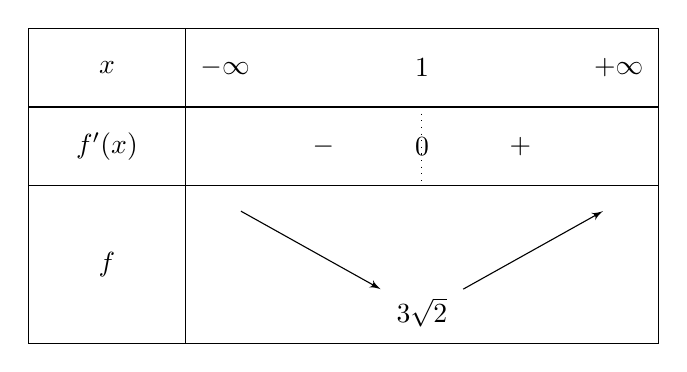
\begin{tikzpicture}[scale=1]
   \tkzTabInit[espcl=2.5]{$x$ / 1 ,$f'(x)$/1, $f$/2}{$-\infty$, $1$ ,$+\infty$}
      \tkzTabLine{ ,-,z,+,  }
      \tkzTabVar{ +/$ $, -/$3\sqrt{2}$, +/$ $}
\end{tikzpicture}
\end{center}

$f$ admet un minimum en 1. Ce minimum vaut $3\sqrt{2}$.
\end{enumerate}
\item D'après la question 1, la distance entre $A$ et un point $M$ de la droite de paramètre $t$ vaut $\sqrt{11t^2-22t+29}$, c'est-à-dire $f(t)$. Cette distance est minimale lorsque $t=1$, c'est-à-dire pour le point de coordonnées $(4,1,0)$ : ce point est donc le projeté orthogonal de $A$ sur la droite $(d)$.
\end{enumerate} \end{solution}



\section*{Exercices de synthèse}

\begin{exercise}
On considère un cube $ABCDEFGH$ de côté de longueur 1. L'espace est alors muni du repère orthonormé $(A;\overrightarrow{AB},\overrightarrow{AD},\overrightarrow{AE})$.
On considère le point $I$, symétrique du point $A$ par rapport au point $C$ ainsi que le point $J$, milieu du segment $[BF]$.

\begin{center}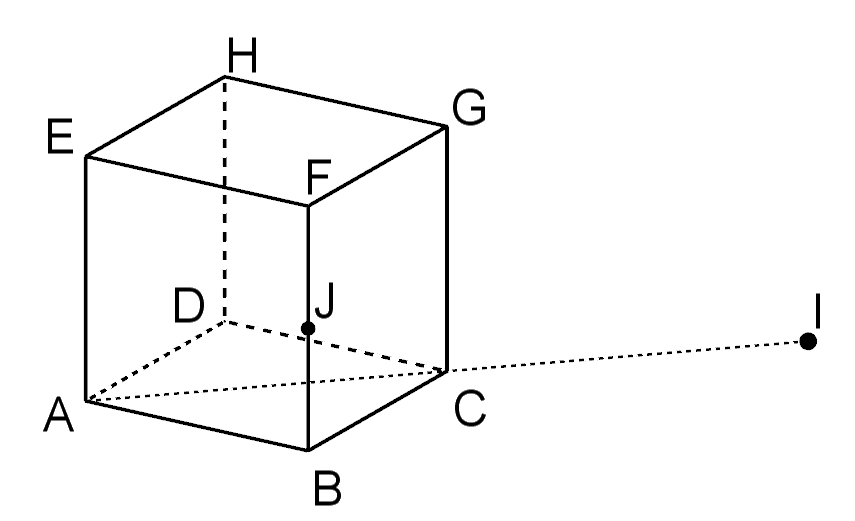
\includegraphics[width=0.5\linewidth]{bb2}\end{center}

\begin{enumerate}
    \item Donner, sans les justifier, les coordonnées des points $I$ et $J$.
    \item Montrer que le vecteur \coorde{n}{1}{-2}{-6} est normal au plan $(IJD)$
    \item En déduire une équation cartésienne du plan $(IJD)$.
    \item Donner une représentation paramétrique de la droite $(BH)$.
    \item Déterminer les coordonnées du point $K$, point d'intersection du plan $(IJD)$ et de la droite $(BH)$.
    \item Calculer $\overrightarrow{KB}\cdot \overrightarrow{KD}$ ainsi que les longueurs $KB$ et $KD$.
    \item En déduire une valeur arrondie au degré près de l'angle $\widehat{BKD}$.
\end{enumerate}
\newpage
\end{exercise}

\begin{solution}\hspace{0pt}
\begin{enumerate}
    \item On a $\overrightarrow{AI}=2\overrightarrow{AC}$. Ainsi, le point $I$ a pour coordonnées $(2,2,0)$. Par ailleurs, $J$ est le milieu de $[BF]$, ses coordonnées sont donc $\left(1;0;\dfrac{1}{2}\right)$.  
    
    \item On a $\coorde{JI}{1}{2}{-1/2}$ et $\coorde{JD}{-1}{1}{-1/2}$. Le repère considéré étant orthonormé, on a alors
    
    \begin{itemize}
    \item $\overrightarrow{JI}\cdot \vec n = 1 \times 1 -2 \times 2 - 6 \times \left(-\dfrac{1}{2}\right)=0$ ;
    \item $\overrightarrow{JD} \cdot \vec n = 1 \times (-1) -2 \times 1 -6 \times \left(-\dfrac{1}{2}\right)=0$.
    \end{itemize}
    Le vecteur $\vec n$ est ainsi orthogonal à deux vecteurs non colinéaires du plan $(IJD)$. Le vecteur \coorde{n}{1}{-2}{-6} est normal au plan $(IJD)$.
    
    \item  Le plan $(IJD)$ passe par le point $I(2,2,0)$ et admet le vecteur \coorde{n}{1}{-2}{-6} comme vecteur normal. Une équation cartésienne de ce plan est donc
    $ 1 \times (x-2) -2 \times (y-2) -6 \times (z-0)=0$
    soit $x-2y-6z+2=0$.
    
    \item La droite $(BH)$ passe par le point $B(1,0,0)$ et admet pour vecteur directeur le vecteur \coorde{BH}{-1}{1}{1}. Une représentation paramétrique de cette droite est donc
    $\left\{\renewcommand{\arraystretch}{1}\renewcommand{\arraystretch}{1}\begin{array}{l}x=1-t\\y=t\\z=t
    
    \end{array}\right.,\quad t \in\mathbb{R}$.
    \item Le point d'intersection du plan $(IJD)$ et de la droite $(BH)$ doit avoir des coordonnées qui vérifient les deux équations. 
    
    Soit $(x,y,z,t)$ quatre réels. On doit avoir $\left\{\renewcommand{\arraystretch}{1}\renewcommand{\arraystretch}{1}\begin{array}{l}x=1-t\\y=t\\z=t\\x-2y-6z+2=0
    \end{array}\right.$.
    
    En utilisant la dernière ligne, on a alors $(1-t)-2t-6t+2=0$ soit $t=\dfrac{1}{3}$. On trouve alors $x=\dfrac{2}{3}$, $y=\dfrac{1}{3}$ et $z=\dfrac{1}{3}$. Réciproquement, on vérifie que le point $K\left(\dfrac{2}{3},\dfrac{1}{3},\dfrac{1}{3}\right)$ vérifient bien les équations du plan $(IJD)$ et de la droite $(BH)$  .
    
    \item  D'une part, 
    \[\overrightarrow{KB}\cdot \overrightarrow{KD} = \left(1-\dfrac{2}{3}\right) \times \left(0-\dfrac{2}{3}\right)+\left(0-\dfrac{1}{3}\right) \times \left(1-\dfrac{1}{3}\right)+\left(0-\dfrac{1}{3}\right)\times \left(0-\dfrac{1}{3}\right)=-\dfrac{1}{3}.\]
    
    Par ailleurs, $\overrightarrow{KB}\cdot \overrightarrow{KD}=KB \times KC \times \cos (\widehat{BKD})$. Or,
    
    \begin{itemize}
    \item $KB = \sqrt{\left(1-\dfrac{2}{3}\right)^2+\left(0-\dfrac{1}{3}\right)^2+\left(0-\dfrac{1}{3}\right)^2}=\dfrac{\sqrt{3}}{3}$ ;
    \item  $KB = \sqrt{\left(0-\dfrac{2}{3}\right)^2+\left(1-\dfrac{1}{3}\right)^2+\left(0-\dfrac{1}{3}\right)^2}=1$.
    \end{itemize}
    
    \item   Ainsi, $ \cos (\widehat{BKD}) = \dfrac{\overrightarrow{KB}\cdot \overrightarrow{KD}}{KB \times KD}=-\dfrac{1}{\sqrt{3}}$.
    
    L'angle $\widehat{BKD}$ mesure environ 125$^{\circ}$.\end{enumerate}
    \end{solution}    

\begin{exercise}[subtitle={(Centres étrangers 2021)}]

Dans un repère orthonormé de l'espace, on considère les points suivants : $A(2 ; -1 ; 0)$ ; $B(3 ; -1 ; 2)$ ; $C(0 ; 4 ; 1)$ et $S(0 ; 1 ; 4)$.

\begin{enumerate}
\item Montrer que le triangle $ABC$ est rectangle en $A$.
\item 
\begin{enumerate}
\item  Montrer que le vecteur  \coorde{n}{2}{1}{-1} est normal au plan $(ABC)$.
\item En déduire une équation cartésienne du plan $(ABC)$.
\item Montrer que les points $A$, $B$, $C$ et $S$ ne sont pas coplanaires.
\end{enumerate}
\vskip5pt
\item Soit $(d)$ la droite orthogonale au plan $(ABC)$ passant par $S$. Elle coupe le plan $ABC$ en $H$.
\begin{enumerate}
\item Déterminer une représentation paramétrique de la droite $(d)$.
\item  Montrer que les coordonnées du point $H$ sont $(2;2;3)$.
\end{enumerate}
\vskip5pt
\item On rappelle que le volume $V$ d'un tétraèdre est $ V = \dfrac{\text{Aire de la base } \times \text{ Hauteur}}{3}$. Calculer le volume du tétraèdre $SABC$.
\vskip5pt
\item \begin{enumerate}
\item Calculer la longueur $SA$.
\item On indique que $SB=\sqrt{17}$. En déduire une mesure de l'angle $\widehat{ASB}$ approchée au dixième de degré.
\end{enumerate}\end{enumerate}
\end{exercise}

\begin{solution}\hspace{0pt}
\begin{enumerate} 
\item On a \coorde{AB}{3-2}{-1-(-1)}{2-0} et \coorde{AC}{0-2}{4-(-1)}{1-0} soit \coorde{AB}{1}{0}{2} et \coorde{AC}{-2}{5}{1}. Puisque le repère est orthonormé, on a
\[ \overrightarrow{AB}\cdot \overrightarrow{AC} = 1 \times (-2) + 0 \times 5 + 2 \times 1 = 0.\]
Ainsi, les droites $(AB)$ et $(AC)$ sont orthogonales. Celles-ci se coupent au point $A$ : ces droites sont donc perpendiculaires et l'angle $\widehat{BAC}$ est donc un angle droit. Le triangle $BAC$ est rectangle en $A$.

\item \begin{enumerate}
\item On a 
\begin{itemize}
\item $\vec n \cdot \overrightarrow{AB}=2 \times 1 + 1 \times 0 + (1-) \times 2 = 0$ ;
\item $\vec n \cdot \overrightarrow{AC}=2\times (-2)+1 \times 5+(-1) \times 1 = 0$.
\end{itemize}
Ainsi, $\vec n$ est orthogonal à deux vecteurs directeurs non colinéaires du plan $(ABC)$, il est donc normal à ce plan.

\item Le plan $(ABC)$ passe par le point $A$ et admet le vecteur $\vec n$ comme vecteur normal. Une équation cartésienne de ce plan est donc
$ 2(x-2)+1(y-(-1))-1(z-0)=0$
soit
$2x+y-z-3=0$.

\item On a $2x_S+y_S-z_S-3=2\times 0 + 1 -4-3=-6\neq 0$. Ainsi, le point $S$ n'appartient pas au plan $(ABC)$ car ses coordonnées ne vérifient pas l'équation de ce plan. Les points $A$, $B$, $C$ et $S$ ne sont pas coplanaires.

\end{enumerate}
\item 
\begin{enumerate}
\item La droite $(d)$ passe par le point $S$ et admet le vecteur $\vec n$ comme vecteur directeur. Une représentation paramétrique de cette droite est donc
\[(d)\quad : \quad \left\{ \renewcommand{\arraystretch}{1}\renewcommand{\arraystretch}{1}\begin{array}{llll}x=&&&2t \\y=&1&+&t\\z=&4&-&t

\end{array}\right.,t\in\mathbb{R}.\]

\item D'une part, les coordonnées du point $H$ vérifient l'équation du plan $(ABC)$. \\En effet, $2\times 2+2-3-3=0$. D'autre part, en prenant $t=1$, on a bien $2t=2$, $1+t=2$ et $4-t=3$. Le point $H$ appartient donc aussi à la droite $(d)$. Il s'agit donc du point d'intersection de $(d)$ et $(ABC)$.

Il est également possible de remplacer $x$, $y$ et $z$ dans l'équation du plan par $2t$, $1+t$ et $4-t$. On trouve alors $t=1$.
\end{enumerate}

\item Prenons le triangle $ABC$ comme base. Le triangle $ABC$ est rectangle en $A$. Son aire vaut donc $\dfrac{AB \times AC}{2}$. Or,
\begin{itemize}
\item $AB= \sqrt{(3-2)^2+(-1-(-1))^2+(2-0)^2}=\sqrt{1+0+4}=\sqrt{5}$ ;
\item $AC=\sqrt{(0-2)^2+(4-(-1))^2+(1-0)^2}=\sqrt{4+25+1}=\sqrt{30}$.
\end{itemize}
Ainsi, l'aire du triangle $ABC$ vaut $\dfrac{\sqrt{5} \times \sqrt{30}}{2}=\dfrac{5\sqrt{6}}{2}$.

D'autre part, $H$ est le projeté orthogonal du point $S$ sur la plan $(ABC)$. $[SH]$ est donc la hauteur du tétraèdre issue du point $S$. Or, $SH = \sqrt{(2-0)^2+(2-1)^2+(3-4)^2}=\sqrt{4+1+1}=\sqrt{6}$.

Ainsi, le volume du tétraèdre $(SABC)$ vaut $ V = \dfrac{1}{3} \times \dfrac{5\sqrt{6}}{2} \times \sqrt{6} = 5$.
\item \begin{enumerate}
\item On a $ SA = \sqrt{(2-0)^2+(-1-1)^2+(0-4)^2}=\sqrt{4+4+16}=\sqrt{24}=2\sqrt{6}$.

\item On a \coorde{SA}{2-0}{-1-1}{0-4} et \coorde{SB}{3-0}{-1-1}{2-4} soit \coorde{SA}{2}{-2}{-4} et \coorde{SB}{3}{-2}{-2}. Ainsi, 
\[ \overrightarrow{SA} \cdot \overrightarrow{SB} = 2 \times 3 -2 \times (-2) -4 \times (-2)=18\]
Or, $ \overrightarrow{SA} \cdot \overrightarrow{SB} = SA \times SB \times \cos \widehat{ASB}$ et donc$ \cos(\widehat{ASB})=\dfrac{\overrightarrow{SA} \cdot \overrightarrow{SB}}{SA \times SB}=\dfrac{18}{\sqrt{17}\times2\sqrt{6}}$.

Ainsi, $\widehat{ASB} \simeq 27,0^{\circ}$.

\end{enumerate}\end{enumerate}\end{solution}



%

    
 

\begin{exercise}Dans l'espace, on considère le cube $ABCDEFGH$ de côtés de longueur 1 représenté ci-dessous.
On note $I$ et $J$ les milieux respectifs des segments $[EH]$ et $[FB]$.

\begin{center}
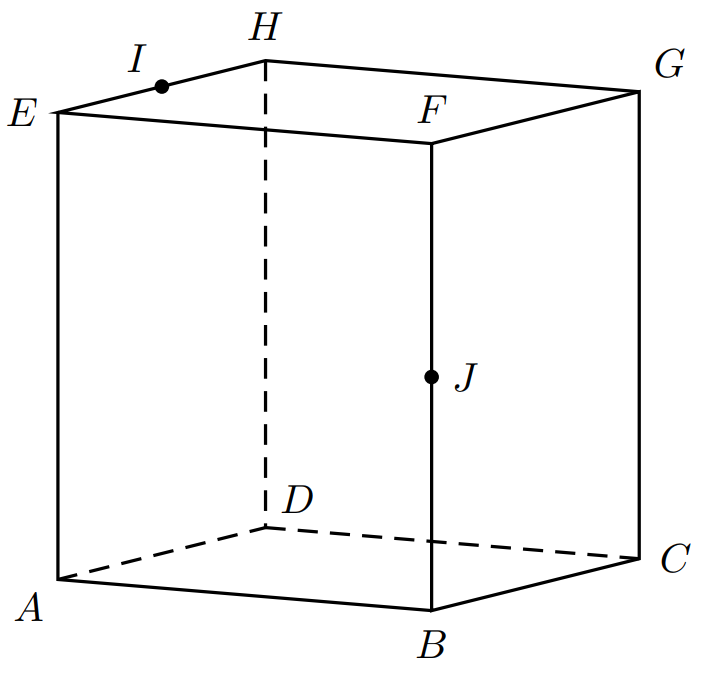
\includegraphics[scale=0.25]{ds5}
\end{center}

L'espace est alors muni du repère orthonormé $(A\, ;\, \overrightarrow{AB}\, , \, \overrightarrow{AD} \, , \, \overrightarrow{AE})$.

\begin{enumerate}
\item Donner, sans les justifier, les coordonnées des points $I$ et $J$.
\vskip5pt
\item \begin{enumerate}
\item Montrer que le vecteur $\vec n \begin{pmatrix} 1 \\ -2 \\ 2 \end{pmatrix}$ est normal au plan $(BGI)$.
\item En déduire une équation cartésienne du plan $(BGI)$.
\item On note $K$ le milieu du segment $[HJ]$. Le point $K$ appartient-il au plan $(BGI)$ ?
\end{enumerate}
\item Le but de cette question est de calculer l'aire du triangle $BGI$.
\begin{enumerate}
\item En utilisant le triangle $FIG$ pour base, montrer que le volume du tétraèdre $FBIG$ vaut $\dfrac{1}{6}$.
\item Déterminer une représentation paramétrique de la droite $\Delta$ passant par $F$ et orthogonale au plan $(BGI)$.
\item La droite $\Delta$ coupe le plan $(BGI)$ en $F'$. Montrer que le point $F'$ a pour coordonnées $\left(\dfrac{7}{9} \, ;\, \dfrac{4}{9} \,;\, \dfrac{5}{9}\right)$.
\item Calculer la longueur $FF'$. En déduire l'aire du triangle $BGI$.
\end{enumerate} \end{enumerate}
\end{exercise}

\begin{solution}\hspace{0pt}
\begin{enumerate}
\item Le point $I$ a pour coordonnées $\left(0 ; \dfrac{1}{2} ; 1\right)$. Le point $J$ a pour coordonnées $\left( 1 ;0 ; \dfrac{1}{2}\right)$.
\vskip5pt
\item \begin{enumerate}
\item Le vecteur $\overrightarrow{BG}$ a pour coordonnées $\begin{pmatrix}0\\1\\1\end{pmatrix} $. Le vecteur $\overrightarrow{BI}$ a pour coordonnées $\begin{pmatrix}-1\\1/2\\1\end{pmatrix} $. Ainsi,
\begin{itemize}
\item $\vec n \cdot \overrightarrow{BG} = 1 \times 0 -2 \times 1 + 2 \times 1 =0$ ;
\item $\vec n \cdot \overrightarrow{BI} = 1 \times (-1) -2 \times 1/2 + 2 \times 1 =0$.\end{itemize}
Le vecteur $\vec n$ est orthogonal a deux vecteurs non colinéaires du plan $(BGI)$. Le vecteur $\vec n \begin{pmatrix} 1 \\ -2 \\ 2 \end{pmatrix}$ est donc normal au plan $(BGI)$.
\item Le point $B(1,0,0)$ appartient au plan $(BGI)$, qui admet le vecteur $\vec n \begin{pmatrix} 1 \\ -2 \\ 2 \end{pmatrix}$ comme vecteur normal. Une équation cartésienne de ce plan est donc $(x-1)-2(y-0)+2(z-0)=0$ soit $x-2y+2z-1=0$.
\vskip5pt
\item On note $K$ le milieu du segment $[HJ]$. Ce point a pour coordonnées $\left(\dfrac{0+1}{2} ; \dfrac{1+0}{2} ; \dfrac{1+\frac{1}{2}}{2}\right)$, c'est-à-dire $\left(\dfrac{1}{2} ; \dfrac{1}{2} ; \dfrac{3}{4}\right)$. Or, $\dfrac{1}{2}-2 \times \dfrac{1}{2}+2 \times \dfrac{3}{4}-1=0$. Les coordonnées du point $K$ vérifient l'équation de $(BGI)$. Le point $K$ appartient donc au plan $(BGI)$.
\end{enumerate}
\vskip10pt
\item Le but de cette question est de calculer l'aire du triangle $BGI$.
\begin{enumerate}
\item Le triangle $FIG$ est isocèle en $I$. Notons $M$ le milieu de $[FG]$. La hauteur issue de $I$ dans le triangle $FIG$ est donc la droite $(IM)$. Il en vient que l'aire de ce triangle vaut $\dfrac{FG \times IM}{2}$ soit $\dfrac{1 \times 1}{2}$.

\begin{center}
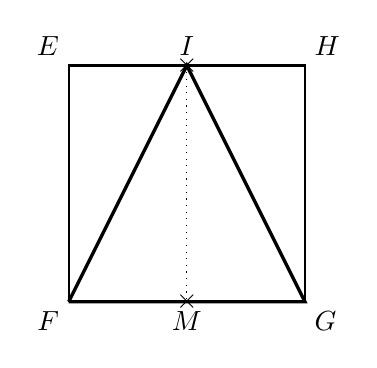
\begin{tikzpicture}[scale = 3]

\draw (0,0) node[below left] {$F$};
\draw (1,0) node[below right] {$G$};
\draw (0,1) node[above left] {$E$};
\draw (1,1) node[above right] {$H$};
\draw (0.5,1) node[above] {$I$};
\draw (0.5,1) node {$\times$};
\draw (0.5,0) node[below] {$M$};
\draw (0.5,0) node {$\times$};
\draw [thick] (0,0) -- (1,0) -- (1,1) -- (0,1) -- (0,0) ;
\draw [very thick] (0,0) -- (1,0) -- (0.5,1) -- (0,0) ;
\draw [dotted] (0.5,1) -- (0.5,0) ;

\end{tikzpicture}
\end{center}
Dans le tétraèdre $FIGB$, la hauteur relative au triangle $FIG$ est $BF$. Ainsi, le volume de ce tétraèdre vaut $\dfrac{\frac{1}{2} \times 1}{3} = \dfrac{1}{6}$.

\vskip5pt
\item La droite $\Delta$ passant par $F(1,0,1)$ et orthogonale au plan $(BGI)$. Elle est donc dirigée par le vecteur $\vec n$. Une représentation paramétrique de cette droite est donc 
\[\left\{\renewcommand{\arraystretch}{1}\renewcommand{\arraystretch}{1}\begin{array}{l} x = 1 + t \\ y=-2t \\ z  = 1+2t\end{array}\right.,\,t\in\mathbb{R}.\]
\vskip5pt
\item La droite $\Delta$ coupe le plan $(BGI)$ en $F'$. On résout

\[\left\{\renewcommand{\arraystretch}{1}\renewcommand{\arraystretch}{1}\begin{array}{l} x = 1 + t \\ y=-2t \\ z  = 1+2t \\ x-2y+2z-1=0 \end{array}\right. \Leftrightarrow \left\{\renewcommand{\arraystretch}{1}\renewcommand{\arraystretch}{1}\begin{array}{l} x = 1 + t \\ y=-2t \\ z  = 1+2t \\ 1+t-2t+2(1+2t)-1=0 \end{array}\right. \Leftrightarrow \left\{\renewcommand{\arraystretch}{1}\renewcommand{\arraystretch}{1}\begin{array}{l}t=-2/9 x = 1 -2/9 \\ y=4/9 \\ z  = 5/9 \end{array}\right. .\]

Le point $F'$ a pour coordonnées $\left(\dfrac{7}{9} \, ;\, \dfrac{4}{9} \,;\, \dfrac{5}{9}\right)$.
\vskip5pt
\item On a

\[FF' = \sqrt{\left(\dfrac{7}{9}-1\right)^2+\left(\dfrac{4}{9}-0\right)^2 + \left(\dfrac{5}{9}-1\right)^2}=\sqrt{ \dfrac{4}{81}+\dfrac{16}{81}+\dfrac{16}{81}}=\sqrt{\dfrac{36}{81}}=\sqrt{\dfrac{4}{9}}=\dfrac{2}{3}.\]

Or, en utilisant le triangle $BGI$ comme base, la hauteur du tétraèdre $FGBI$ relative à cette base n'est autre que $(FF')$. Si on note $A_{BGI}$ l'aire du triangle $(BGI)$, il en vient que le volume du tétraèdre vaut $\dfrac{A_{BGI} \times FF'}{3}$ soit $\dfrac{2A_{BGI}}{9}$. Or, d'après les questions précédentes, ce volume vaut $\dfrac{1}{6}$. Ainsi, $A_{BGI}= \dfrac{1}{6} \times \dfrac{9}{2} = \dfrac{3}{4}$ .
\end{enumerate} \end{enumerate}\end{solution}


\chapter{Corrigés}


\printsolutions[headings={false} ]




\end{document}